\chapter{LOGIQUE ET PHILOSOPHIE DU LANGAGE}
\label{chapter-4}
\markright{Logique et philosophie du langage}
\origpage{85}{071}
\begin{keybox}[Plan du chapitre]
\small
\textbf{I.\quad LA LOGIQUE : SCIENCE DE L’INFÉRENCE}
\begin{enumerate}[label=\arabic*.]
\item Les différents types de raisonnement
\begin{enumerate}[label=\textcircled{\scriptsize\arabic*}]
\item Raisonnement formalisé et raisonnement non formalisé
\item Raisonnement \textit{a priori} et raisonnement \textit{a posteriori}
\end{enumerate}
\item Les trois types d’inférence
\begin{enumerate}[label=\textcircled{\scriptsize\arabic*}]
\item La déduction
\item L’induction
\item L’abduction
\end{enumerate}
\end{enumerate}
\textbf{II.\quad LES LIMITES ENTRE LOGIQUE ET LANGAGE}
\begin{enumerate}[label=\arabic*.]
\item Le paralogisme
\begin{enumerate}[label=\textcircled{\scriptsize\arabic*}]
\item L’affirmation du conséquent
\item La négation de l’antécédent
\item Le \textit{non sequitur}
\end{enumerate}
\item Les sophismes
\item Les paradoxes et antilogies
\begin{enumerate}[label=\textcircled{\scriptsize\arabic*}]
\item Épiménide : le paradoxe du menteur
\item Lucien de Samosate : le paradoxe du crocodile
\item Sextus Empiricus : le paradoxe de l’avocat
\item Bertrand Russell : le paradoxe du barbier
\end{enumerate}
\end{enumerate}
\textbf{III. LA LOGIQUE D’ARISTOTE : LA SCIENCE DU \textit{LOGOS}}
\begin{enumerate}[label=\arabic*.]
\item L’\textit{Organon}
\item \textit{Les Catégories}
\begin{enumerate}[label=\textcircled{\scriptsize\arabic*}]
\item Sujet et prédicat
\item La copule
\item Thème et rhème
\begin{enumerate}[label=\arabic*.]
\item Le thème
\item Rhème et rhématisation
\end{enumerate}
\origpage{86}{072}
\item Les trois principes d’Aristote
\begin{enumerate}[label=\arabic*.]
\item Le principe de non-contradiction
\item Le principe du tiers exclu
\item Le principe d’identité
\end{enumerate}
\end{enumerate}
\item \textit{De l’interprétation}
\begin{enumerate}[label=\textcircled{\scriptsize\arabic*}]
\item Le carré logique
\item Illustration
\end{enumerate}
\item Les \textit{Premiers Analytiques}
\begin{enumerate}[label=\textcircled{\scriptsize\arabic*}]
\item Le syllogisme
\begin{enumerate}[label=\arabic*.]
\item Les propositions
\item Vérité et validité
\end{enumerate}
\item L’enthymème
\item L’épichérème
\end{enumerate}
\item \textit{Isagoge}, de Porphyre
\begin{enumerate}[label=\textcircled{\scriptsize\arabic*}]
\item Les cinq universaux
\item L’arbre de Porphyre
\item La question des « universaux »
\end{enumerate}
\end{enumerate}
\textbf{IV. PHILOSOPHIE MÉDIÉVALE : LA « QUERELLE DES UNIVERSAUX »}
\begin{enumerate}[label=\arabic*.]
\item Le nominalisme
\begin{enumerate}[label=\textcircled{\scriptsize\arabic*}]
\item Roscelin de Compiègne
\item Jean Buridan
\item Guillaume d’Ockham
\begin{enumerate}[label=\arabic*.]
\item Un précurseur de la philosophie du langage
\item Le rasoir d’Ockham
\end{enumerate}
\end{enumerate}
\item Le réalisme
\begin{enumerate}[label=\textcircled{\scriptsize\arabic*}]
\item Guillaume de Champeaux
\item La thèse conceptualiste : Pierre Abélard
\end{enumerate}
\end{enumerate}
\textbf{V.\quad LA PÉRIODE MODERNE : LA RUPTURE ÉPISTÉMOLOGIQUE}
\begin{enumerate}[label=\arabic*.]
\item Gottlob FREGE : naissance de la logique moderne
\begin{enumerate}[label=\textcircled{\scriptsize\arabic*}]
\item \textit{Que la science justifie le recours à une idéographie} (1882)
\item \textit{Sens et dénotation} (1892)
\begin{enumerate}[label=\arabic*.]
\item La dénotation
\item Le sens
\item L’intension et extension
\end{enumerate}
\end{enumerate}
\origpage{87}{073}
\item Bertrand Russel : naissance de la philosophie analytique
\begin{enumerate}[label=\textcircled{\scriptsize\arabic*}]
\item Le paradoxe de Russel
\begin{enumerate}[label=\arabic*.]
\item Formulation du paradoxe
\item La théorie des types
\end{enumerate}
\item \textit{On denoting} (1905)
\begin{enumerate}[label=\arabic*.]
\item « Le roi de France est chauve. »
\item La résolution de l’énigme
\end{enumerate}
\item Russell et Oswald Ducrot : Posé, présupposé et sous-entendu
\item Russell et Gongsun Long : 白马非马
\item Russell et Zhuangzi : 鱼之乐
\end{enumerate}
\item Ludwig von Wittgenstein : les limites du langage
\begin{enumerate}[label=\textcircled{\scriptsize\arabic*}]
\item Le \textit{Tractatus logico-philosophicus}
\begin{enumerate}[label=\arabic*.]
\item L’atomisme logique
\item Le fait et l’objet
\item Le sens
\item Les différents types de propositions
\begin{enumerate}[label=\arabic*)]
\item Les propositions pourvues de sens
\item Les propositions vides de sens
\item Les propositions dépourvues de sens
\end{enumerate}
\item La philosophie comme « critique du langage »
\end{enumerate}
\item La « seconde philosophie » de Wittgenstein
\begin{enumerate}[label=\arabic*.]
\item La philosophie linguistique : retour au langage ordinaire
\item La signification par l’usage
\item Les jeux de langage
\end{enumerate}
\end{enumerate}
\item Le Cercle de Vienne : le positivisme logique
\begin{enumerate}[label=\textcircled{\scriptsize\arabic*}]
\item La théorie vérificationniste
\item La critique de la métaphysique
\end{enumerate}
\end{enumerate}
\textbf{Exercices}\par
\textbf{Pour aller plus loin}\par
\textbf{Glossaire}
\end{keybox}
\clearpage
\origpage{88}{074}
\lecturetitle{Introduction}
Le \textit{Dictionnaire de la langue française} d’Émile Littré définit la logique comme la « science du raisonnement ». Cela ne nous étonnera pas, car nous savons depuis le premier chapitre que le mot « logique » nous vient du grec \textit{logos} qui signifie à la fois « langage », et « raison ». Si l’on se base sur cette étymologie, et du fait de cette identité entre langage et raison, on peut dire que la première science du langage, c’est la logique. Impossible de traiter de linguistique, donc, sans évoquer son lointain parent, la logique.

Définie comme un « art de penser » par les solitaires de Port Royal, la logique ne se définit pas seulement par son objet, à savoir la pensée, le langage, et leurs rapports réciproques, mais aussi encore par son but : la recherche de la vérité. C’est ce qui la distingue de la dialectique, art du dialogue (\textit{dialogos}) qui ne raisonne pas mais argumente, et qu’Emmanuel Kant (1724-1804) assimile dans \textit{Critique de la raison pure} (1787) à une « logique de l’apparence ». En prenant en considération son objet et son but, on dira que la logique est la science des conditions que la \textit{pensée} doit remplir pour que les énoncés du \textit{langage soient vrais}.\ednote{应区分推理有效性与命题事实真值：有效推理保证的是“若前提真，则结论真”，单凭形式正确不能保证前提或结论实际为真。下文原书第 090 页亦区分 vérité 与 validité；此处定义不宜理解为逻辑形式本身足以确保事实真理。}

Quant aux problèmes philosophiques posés par le langage, ils ont eux aussi fait l’objet des investigations de Platon, d’Aristote, mais aussi de la philosophie médiévale et classique. Le début du 20\textsuperscript{e} siècle a vu se produire une rupture épistémologique, et la « science du logos » s’est scindée en deux sciences distinctes : la logique formelle (science du raisonnement) d’une part, et la linguistique (science du langage) d’autre part. Au même moment, une nouvelle discipline a vu le jour au sein de la philosophie du langage : la philosophie analytique, essentiellement anglo-saxonne, qui, constatant les limites de notre langage naturel, à savoir celui que vous et moi utilisons au quotidien, a introduit la logique en philosophie afin de « clarifier la pensée ». Comme l’a dit André Gide, « L’illogisme irrite. Trop de logique ennuie ». Dans ce chapitre, je tenterai d’éviter ces deux écueils.

\section{LA LOGIQUE : SCIENCE DE L’INFÉRENCE}
En logique, l’inférence est un mouvement de la pensée allant des principes à la conclusion. La logique peut donc être définie comme l’étude de l’inférence, terme générique recouvrant plusieurs types de raisonnement.

\subsection{Les différents types de raisonnement}
Le mécanisme d’élaboration de ces inférences est le raisonnement. On peut distinguer plusieurs types de raisonnement.

\subsubsection*{\textcircled{\scriptsize 1} Raisonnement formalisé et raisonnement non formalisé}
Un raisonnement est formalisé s’il s’énonce dans une langue formelle qui obéit à des règles
\origcont{89}{075}
de syntaxe strictes et évite les ambiguïtés sémantiques. Typiquement, les raisonnements mathématiques sont des raisonnements formalisés. C’est le cas par exemple de la célèbre loi sur la relativité restreinte formulée par Albert Einstein en 1905 : $E=mc^2$.

Un raisonnement peut également être non formalisé, c’est-à-dire exprimé en langue naturelle. Voici la même loi sur la relativité exprimée en langue naturel.\ednote{原文 naturel 与阴性名词 langue 不一致，应作 naturelle。另，单列一个公式或其自然语言表达尚不构成有前提和结论的完整“推理”；这两个例子直接展示的是表达方式的区别。}

Ex : une particule de masse (m) possède une énergie (E) dont la valeur est donnée par le produit de (m) par le carré de la vitesse de la lumière (c).

La philosophie recourt essentiellement aux raisonnements non formalisés. Cela n’est pas sans conséquence, et nous y reviendrons en fin de chapitre.

\subsubsection*{\textcircled{\scriptsize 2} Raisonnement \textit{a priori} et raisonnement \textit{a posteriori}}
Le raisonnement \textit{a priori} (dit aussi « analytique »)\ednote{“a priori”与“analytique”不是同义词，尤其不能在 Kant 的论述中等同。前者涉及认识是否独立于经验，后者涉及判断中谓词与主词概念的关系；Kant 明确讨论“先天综合判断”。见 \ecite{18}，导论 IV–VI。} recourt souvent à une formalisation logique pour établir une preuve. Il repose surtout sur des principes et sur une analyse conceptuelle. Dans la pensée de \textbf{Kant}, c’est une connaissance indépendante de l’expérience. Par exemple, si A=B et B=C, alors A=C. Un autre exemple intéressant est celui du chiliogone, polygone à 1000 côtés, utilisé en philosophie, en particulier par \textbf{Descartes}, pour désigner quelque chose qui est impossible à voir clairement et distinctement, mais facile à concevoir dans l’idée, donc a priori.

\begin{lecture}{Lecture : \textit{Méditations métaphysiques} (extrait)}
Par exemple, lorsque j’imagine un triangle, non seulement je conçois que c’est une figure composée de trois lignes, mais avec cela j’envisage ces trois lignes comme présentes par la force et l’application intérieure de mon esprit ; et c’est proprement ce que j’appelle imaginer. Que si je veux penser à un chiliogone, je conçois bien à la vérité que c’est une figure composée de mille côtés aussi facilement que je conçois qu’un triangle est une figure composée de trois côtés seulement ; mais je ne puis pas imaginer les mille côtés d’un chiliogone comme je fais les trois d’un triangle, ni pour ainsi dire les regarder comme présents avec les yeux de mon esprit.
\end{lecture}

À l’opposé, il existe des raisonnements \textit{a posteriori} reposant sur des « données empiriques » recueillies par expérimentation ou observation. Dans un article de la Logique de Port-Royal, intitulé « Des diverses manières de mal raisonner, que l’on appelle sophismes », les auteurs en donnent l’exemple suivant :

\begin{adjustwidth}{4mm}{4mm}\small\itshape
Par exemple, lorsqu’on a éprouvé sur beaucoup de mers que l’eau en est salée, et sur beaucoup de rivières que l’eau en est douce, on conclut généralement que l’eau de la mer est salée, et celle des rivières douces.
\end{adjustwidth}

\origpage{90}{076}
\subsection{Les trois types d’inférence}
Pendant des siècles, on a distingué deux types d’inférence : l’inférence déductive et l’inférence inductive. Au 19\textsuperscript{e} siècle, le philosophe et logicien \textbf{Charles Sanders Peirce} (1839-1914) a introduit les inférences abductives. On distingue dès lors trois types d’inférence : la déduction (raisonnement logique), l’induction (raisonnement statistique) et l’abduction (inférence qui mène à la découverte d’une hypothèse plausible).

\subsubsection*{\textcircled{\scriptsize 1} La déduction}
Dans notre langage de tous les jours, la déduction est l’action de tirer une conséquence logique de quelque chose, par un raisonnement. En logique, c’est la méthode par laquelle on va de la cause aux effets, du principe aux conséquences, du général au particulier. La déduction logique est constituée d’un enchaînement de propositions qui respectent des règles définies, et sans recours à l’expérience : c’est donc un raisonnement formalisé et \textit{a priori}.\ednote{演绎并不必然是“从原因到结果”或“从一般到个别”，也不要求以形式语言写出。由“A 且 B”推出“A”就是反例；经验获得的前提也可用于演绎。应更正为：演绎有效性要求不存在前提全真而结论假的情形。} Ce type de raisonnement, théorisé très tôt par Aristote trouve son application la plus connue dans le syllogisme, sur lequel nous allons revenir en détail dans un instant. Dans la déduction, la validité du raisonnement est liée au respect de la forme du raisonnement : la conclusion peut être fausse si l’une des prémisses est fausse, mais elle est nécessairement vraie si les prémisses sont vraies. Le raisonnement déductif est le seul moyen de preuve par la logique. Il permet d’expliciter ce qui était latent, mais n’apporte pas de connaissance nouvelle. Nous verrons que cela le différencie de l’abduction.
\begin{center}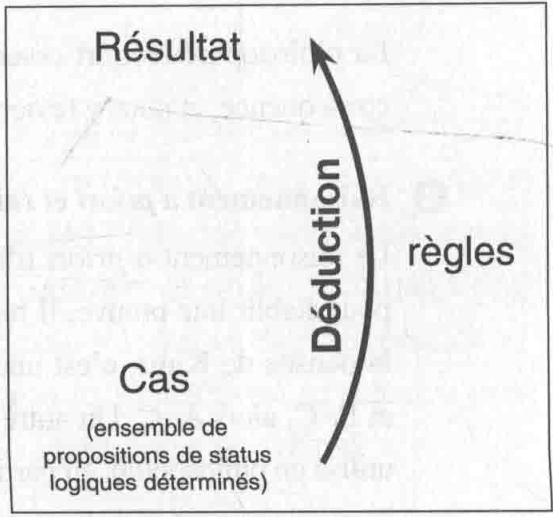
\includegraphics[width=49mm]{assets/ch04_deduction_original.png}\end{center}

Prenons un exemple. Un haricot est tiré d’une boîte. Une règle, connue au préalable, énonce que tous les haricots de la boîte sont blancs. Le résultat, naturellement, est que le haricot est blanc. Plus exactement, le haricot tiré de la boîte (le cas) est blanc parce qu’on lui applique une règle qui énonce que tous les haricots de la boîte sont blancs.

\subsubsection*{\textcircled{\scriptsize 2} L’induction}
L’induction est un genre de raisonnement qui se propose de trouver des lois générales à partir de l’observation de faits particuliers sur une base probabiliste. À l’inverse de la déduction, elle est un type de raisonnement \textit{a posteriori} où l’on part de cas individuels pour accéder aux énoncés universels. Ce type de raisonnement s’appuie donc sur la vérification répétée d’un fait. Par exemple, si tous les corbeaux que l’on voit sont noirs et que l’on n’a encore jamais
\origcont{91}{077}
rencontré de corbeaux d’une autre couleur, on induira alors la loi générale selon laquelle tous les corbeaux sont noirs. Autre différence avec la déduction qui permet d’obtenir la vérité, l’induction ne nous permet d’obtenir qu’une quasi-certitude, et le premier contre-exemple (par exemple, un corbeau blanc) mettra en cause la loi précédemment établie, qui s’avèrera donc fausse. Pas de vérité absolue ici donc, mais une loi basée sur des statistiques. Ce mode de raisonnement n’est donc pas sans poser des problèmes.
\begin{center}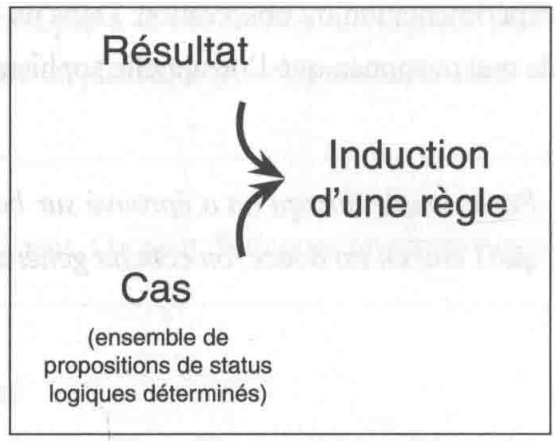
\includegraphics[width=49mm]{assets/ch04_induction_original.png}\end{center}

Reprenons notre boîte de haricots et faisons une expérience. On part cette fois-ci du cas et du résultat. Un haricot est tiré de la boîte N° 2. Résultat : il est rouge. On peut éventuellement multiplier le nombre de tirages. Le deuxième haricot tiré de la boîte N° 2 et lui aussi rouge,\ednote{原文 et 应作 est：“Le deuxième haricot […] est lui aussi rouge”。} ainsi que le troisième, le quatrième etc. On peut formuler une règle qui est que tous les haricots de la boîte N° 2 sont rouges, comme suit :

\subsubsection*{\textcircled{\scriptsize 3} L’abduction}
L’abduction est un mode de raisonnement parfois désigné comme une « inférence de la meilleure explication ». Il s’agit en effet, lorsque l’on observe un fait dont on connaît une cause \textit{possible}, de conclure à titre d’\textit{hypothèse} que ce fait est probablement dû à cette cause-ci. Précisons que l’hypothèse, par définition, n’est pas vraie mais vraisemblable.\ednote{假说并非“按定义不真”；其真值尚未由当前证据确立，可以为真，也可以为假。应作“尚未证实，而被认为具有一定可信性”。同页“comme suit :”之后未见归纳例子的续式，故不擅补。} L’invention fortuite du micro-onde par \textbf{Percy Spencer} (1884-1970) en 1945 est un exemple d’abduction : alors qu’il travaillait dans son laboratoire à proximité d’un magnétron (appareil produisant des ondes électromagnétiques), il s’est aperçu que les bonbons au chocolat qui se trouvaient dans la poche de sa chemise avaient fondu. En l’absence d’autre explication possible, il a fait l’abduction suivante : les bonbons avaient été réchauffés par les ondes du magnétron. A travers cet exemple, on voit que l’abduction consiste à choisir la ou les hypothèses les plus vraisemblables et à éliminer les plus improbables pour expliquer un phénomène donné, puis aboutir ensuite par déduction à une conclusion probable (mais pas certaine) qui concorde avec les observations. Spencer avait observé un fait (le chocolat fondu dans la poche), et en a tiré l’hypothèse la plus probable : les ondes émises par le magnétron l’avaient fait fondre.
\begin{center}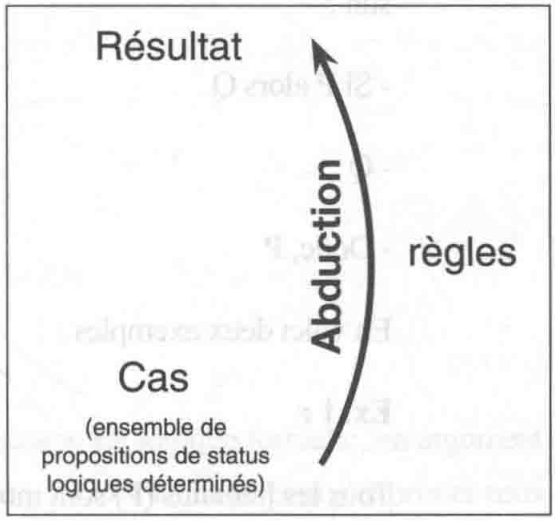
\includegraphics[width=49mm]{assets/ch04_abduction_original.png}\end{center}

Revenons à nos haricots. Dans notre troisième expérience, le haricot que nous tirons est blanc. D’où provient-il ? Si l’on connaît une règle disant : il y a des haricots blancs dans la boîte N° 1, on peut imaginer un cas qui est que le haricot en question provient bien de la boîte N° 1.

\section{LES LIMITES ENTRE LOGIQUE ET LANGAGE}
On a longtemps considéré que tout énoncé est, par nature, logique. Or, ce n’est pas le cas : les lois du langage et les lois de la logique ne sont pas identiques, et des raisonnements qui en apparence sont rigoureusement
\origcont{92}{078}
logiques aboutissent à des conclusions absurdes et qui vont à l’encontre le bon sens.\ednote{à l’encontre 后应接 de，故“à l’encontre le bon sens”应作“à l’encontre du bon sens”。} Ces raisonnements non valides peuvent être regroupés en deux familles : les paralogismes et les sophismes. La distinction entre les deux ne concerne pas la logique à proprement parler, plutôt la rhétorique : un sophisme est en effet un paralogisme volontaire lié à une mauvaise intention. Cette différence est du même type que celle de l’erreur et du mensonge.

\subsection{Le paralogisme}
Un paralogisme est un raisonnement faux qui a l’apparence de la rigueur logique, et dans lequel le locuteur est de bonne foi. Il existe trois types de paralogismes formels :\ednote{下列 non sequitur 并非与前两者互不相交的第三种形式：作者在该节列出的两式正是肯定后件与否定前件。宜将此句理解并更正为“这里讨论以下形式及其总称”，而非穷尽形式谬误的三分法。}

\subsubsection*{\textcircled{\scriptsize 1} L’affirmation du conséquent}
L’affirmation du conséquent est un paralogisme formel dans lequel on considère une condition suffisante comme une condition nécessaire. En langage naturel, ce paralogisme s’exprime comme suit :
\begin{itemize}[label=--]
\item Si P alors Q
\item Q
\item Donc, P
\end{itemize}
En voici deux exemples :

\minititle{Ex. 1 :}
Tous les humains (P) sont mortels (Q).

Un âne est mortel (Q).

Donc un âne est un humain (P).

L’affirmation du conséquent consiste ici à conclure qu’un cas particulier (la catégorie âne) fait partie d’une catégorie générale (humain) du seul fait qu’ils partagent une propriété (mortel).

\minititle{Ex. 2 :}
S’il a plu (P), alors le sol est mouillé (Q).

Le sol est mouillé (Q).

Donc il a plu (P).

Il est bien évident que le sol peut être mouillé par d’autres raisons que la pluie. Par exemple, les larmes que vous versez à la lecture de ce chapitre bien difficile.

\subsubsection*{\textcircled{\scriptsize 2} La négation de l’antécédent}
La négation de l’antécédent est un paralogisme formel qui consiste à nier une propriété particulière pour un cas particulier, sous prétexte qu’il n’appartient pas à la catégorie générale qui possède cette
\origcont{93}{079}
propriété. Il s’exprime comme suit :
\begin{itemize}[label=--]
\item Si P alors Q
\item Il est faux que P
\item Donc il est faux que Q
\end{itemize}
En voici deux exemples :

\minititle{Ex. 1 :}
Tous les humains sont mortels

Un âne n’est pas un humain

Donc un âne est immortel

\minititle{Ex. 2 :}
S’il a plu (P) alors le sol est mouillé (Q)

Il n’a pas plu (il est faux que P)

Donc le sol n’est pas mouillé (il est faux que Q)

\subsubsection*{\textcircled{\scriptsize 3} Le \textit{non sequitur}}
\textit{Non sequitur} signifie, en latin, « qui ne suit pas les prémisses ». En logique formelle, un argument est un \textit{non sequitur} si la conclusion ne suit pas les prémisses. Le \textit{non sequitur} peut s’exprimer sous les formes suivantes :
\begin{itemize}[label=--]
\item Si A est vraie, alors B est vraie.
\item B est vraie.
\item Donc, A doit être vraie.
\end{itemize}
\minititle{Ex :}
Si je suis à Tokyo (A), alors je suis au Japon (B).

Je suis au Japon.

Donc, je dois être à Tokyo.

\begin{itemize}[label=--]
\item Si A est vraie, alors B est vraie.
\item A est fausse.
\item Donc, B est fausse.
\end{itemize}

\origpage{94}{080}
\minititle{Ex :}
Si je suis à Tokyo (A), alors je suis au Japon (B).

Je ne suis pas à Tokyo.

Donc, je ne suis pas au Japon.

\subsection{Les sophismes}
Le sophisme, comme le paralogisme, est une argumentation à la logique fallacieuse, mais à la différence du paralogisme, le sophisme est prononcé avec l’intention de convaincre, voire tromper l’auditoire afin de prendre l’avantage dans une discussion ou un débat. En voici un exemple :

\minititle{Ex :}
Tout ce qui est rare est cher.

Un diamant bon marché est rare.

Donc un diamant bon marché est cher.\ednote{若三个句子中的“rare”“cher”取相同含义，且将第一个全称前提视为真，形式本身是有效的。问题在大前提并非普遍真实，或“rare”的使用发生偷换，不宜把本例当成单纯的形式无效。原例保留。}

\subsection{Les paradoxes et antilogies}
Le \textit{Dictionnaire de l’Académie française} définit un paradoxe (du grec \textit{para}, « contre », et \textit{doxa}, « opinion ») comme « une proposition qui, énonçant son propre contraire, paraît à la fois vraie et fausse ; raisonnement dont la conclusion contredit les prémisses ou qui engendre deux conclusions contradictoires ». Il faut le distinguer de l’antilogie, qui est une contradiction entre deux ou plusieurs idées au sein d’un discours, d’un texte, d’une opinion voire d’une théorie scientifique ou philosophique.

\subsubsection*{\textcircled{\scriptsize 1} Épiménide : le paradoxe du menteur}
Le paradoxe du menteur (ou plutôt « antilogie » ici) aurait été inventé par un adversaire d’Aristote, le logicien \textbf{Eubulide de Milet}, vers 350 avant J.C. Sous sa forme la plus concise, il s’énonce ainsi : un homme déclare : « Je mens. ». Si c’est vrai, c’est faux. Si c’est faux, c’est vrai. Le paradoxe d’Eubulide est dérivé d’un autre paradoxe, le « paradoxe du Crétois » (appelé aussi « paradoxe d’Épiménide ») formulé par poète crétois \textbf{Épiménide} (7\textsuperscript{e} siècle avant J.-C.) qui aurait affirmé : « Tous les Crétois sont des menteurs. » Épiménide est crétois, donc il ment. S’il ment, il dit effectivement la vérité.\ednote{此步推论不成立。“并非所有克里特人都说谎”只要求存在一个反例，不推出 Épiménide 本人的当前发言为真；“说谎者”也不等于每句话都为假。严格的说谎者悖论须将语句明确自指为“本句为假”，不能直接以这里的全称陈述代替。另，“formulé par poète crétois”缺冠词，应为“par le poète crétois”。} L’énoncé est à la fois vrai et faux, ce qui viole le principe de non-contradiction.

\subsubsection*{\textcircled{\scriptsize 2} Lucien de Samosate : le paradoxe du crocodile}
Le rhéteur \textbf{Lucien de Samosate} (120-180) a proposé un paradoxe auto-référentiel de la même famille que celui du menteur. Un crocodile s’empare d’un bébé et dit à la mère : « Si tu devines ce que je vais faire, je te rends le bébé, sinon je le dévore ». En supposant que le crocodile tienne parole, que doit dire la mère pour que le crocodile rende l’enfant à sa mère ? Une réponse usuelle
\origcont{95}{081}
de la mère est : « Tu vas le dévorer ! » Si le crocodile dévore en effet le bébé, la mère a bien deviné et le crocodile doit rendre le bébé. Mais si le crocodile ne dévore pas le bébé, la mère s’est trompée et le crocodile doit dévorer le bébé. Ce paradoxe est similaire au paradoxe du menteur, dans le sens où si l’on veut que l’affirmation soit vraie, elle devient fausse et si on veut qu’elle soit fausse, elle devient vraie.

\subsubsection*{\textcircled{\scriptsize 3} Sextus Empiricus : le paradoxe de l’avocat}
Le paradoxe de l’avocat est un paradoxe logique de la Grèce antique que l’on trouve dans le traité « Contre les rhéteurs » de \textbf{Sextus Empiricus}. Il met en scène un conflit entre le sophiste \textbf{Protagoras} et \textbf{Euathlos}, un de ses élèves. Euathlos était pauvre et ne pouvait payer les leçons de Protagoras. Celui-ci l’a accepté comme disciple après avoir conclu l’accord suivant : Euathlos rembourserait les leçons reçues une fois qu’il aurait gagné son premier procès. Une fois son enseignement terminé, Euathlos a refusé à la fois de plaider comme avocat et de payer Protagoras. Faute de plaider, il ne pouvait gagner aucun procès. N’ayant pas gagné de procès, il n’avait pas à rembourser son maître. Protagoras l’a alors attaqué en justice afin de l’obliger à plaider. Le raisonnement de Protagoras était le suivant : si Euathlos gagne son procès, il devra me rembourser, car c’est les termes de notre accord. Si Euathlos perd son procès, il devra aussi me rembourser, car la justice l’y contraindra. Protagoras serait donc remboursé quelle que soit l’issue du procès. Soit en vertu de l’accord passé avec Euathlos, soit par une décision de justice. Le paradoxe est intervenu lors de la réponse de Euathlos, qui a décidé d’utiliser un argument presque identique à celui de son maître, mais cette fois dans le but de se faire acquitter. Quelle que soit l’issue du procès, Euathlos considérait qu’il n’aurait rien à payer. En effet, s’il gagnait son procès, il ne devrait pas rembourser son maître, puisque la justice l’aurait blanchi. Mais s’il perdait son procès, alors il ne devrait pas rembourser son maître, puisque les leçons de ce dernier auraient été inefficaces. Encore une fois, c’est un paradoxe auto-référentiel classique, du type du menteur.

\subsubsection*{\textcircled{\scriptsize 4} Bertrand Russell : le paradoxe du barbier}
Le paradoxe du barbier est un paradoxe à but didactique formulé par Bertrand Russell vers 1901 et publié en 1903.\ednote{这里应区分集合论的 Russell 悖论与理发师故事的具体表述；正文将两者的年代直接合并。此次未完成理发师故事最早版本的文献核定，暂保留年份为待核，不据集合论悖论的发表年替故事定年。} Le conseil municipal d’un village vote un arrêté municipal qui enjoint à son barbier de raser tous les habitants masculins du village qui ne se rasent pas eux-mêmes et seulement ceux-ci. Le barbier, qui est bien un habitant du village, n’a pas pu respecter cette règle. En effet, s’il se rase lui-même, il enfreint la règle, car le barbier ne peut raser que les hommes qui ne se rasent pas eux-mêmes. Mais s’il ne se rase pas lui-même, s’il se fait raser par quelqu’un d’autre, il est en tort également, car il a la charge de raser les hommes qui ne se rasent pas eux-mêmes, donc lui-même. On peut formuler le paradoxe ainsi : l’ensemble des ensembles n’appartenant pas à eux-mêmes appartient-il à lui-même ? Si on répond oui, alors, comme par définition les membres de cet ensemble n’appartiennent pas à eux-mêmes, il n’appartient pas à lui-même, ce qui est une contradiction. Mais si on répond non, il a alors la propriété requise pour appartenir à lui-même, et c’est une nouvelle contradiction.

Les différents paradoxes présentés ci-dessus montrent clairement que le langage naturel n’est pas
\origcont{96}{082}
adapté à la pensée logique et aux sciences abstraites en général. Cette imperfection, source d’erreurs d’interprétation, a fait l’objet d’intenses réflexions à l’époque moderne qui ont donné naissance à la logique moderne.\ednote{“这些悖论证明自然语言不适于逻辑思考”并不由前例推出。集合论悖论可直接形式化为 $R\in R\leftrightarrow R\notin R$；理发师条件也可形式化。因此矛盾不能仅归因于自然语言，应检查有关定义、公理或语义假设。}

\section{LA LOGIQUE D’ARISTOTE : LA SCIENCE DU \textit{LOGOS}}
On s’accorde à faire commencer l’histoire de la logique avec les six traités de logique d’Aristote qui ont ultérieurement été rassemblés sous le titre commun d’\textit{Organon} (en grec ancien, « outil » ou « instrument »).

\subsection{L’\textit{Organon}}
Le titre d’\textit{Organon} n’est pas d’Aristote. Il est mentionné pour la première fois par \textbf{Diogène Laërce}, poète et biographe du début du IIIe siècle et auteur d’un célèbre \textit{Vies, doctrines et sentences des philosophes illustres}. Le fait d’utiliser le terme d’« instrument » pour désigner ces traités de logique n’est pas neutre : pour Aristote et ses successeurs, l’étude de la logique n’était qu’un outil de préparation à la philosophie, une propédeutique (une science préalable) à toute pensée rationnelle. C’est en ce sens qu’Aristote a écrit dans sa \textit{Métaphysique} : « Il faut connaître les \textit{Analytiques} avant d’aborder aucune science », les \textit{Analytiques} étant deux livres essentiels de la logique d’Aristote.

La composition précise de l’\textit{Organon} a varié selon les commentateurs, certains ayant voulu y inclure la \textit{Rhétorique} et la \textit{Poétique}. De nos jours, selon la catégorisation retenue, l’\textit{Organon} comprend :
\begin{itemize}
\item \textit{Les catégories}
\item \textit{De l’interprétation}
\item \textit{Les premiers analytiques}
\item \textit{Les seconds analytiques}
\item \textit{Les topiques}
\item \textit{Les réfutations sophistiques}
\end{itemize}
On considère que c’est avec \textit{De l’interprétation} et les \textit{Premiers Analytiques} qu’Aristote crée la logique.

\subsection{\textit{Les Catégories}}
\textit{Les Catégories} se trouvent placées en tête de l’\textit{Organon}. Aristote y développe les bases de sa logique et de son ontologie (la science de l’être) en étudiant la façon dont le langage peut désigner et signifier « ce qui est ». Pour Aristote, le langage est par définition une expression adéquate de la raison. Les mots reflètent les différents « modes d’être » auxquels se réduit toute réalité. Ces modes d’être (les \textit{modus essendi} des grammairiens modistes) sont au nombre de dix et constituent les catégories (en grec, \textit{categorein}, « accuser »). Dans la terminologie aristotélicienne, les catégories seront donc les « modes d’accusation » de l’être. Dans une hiérarchie qui part des « individus » pour arriver aux « genres » en passant par les « espèces », les « catégories » sont les genres les plus généraux de l’être.

\origpage{97}{083}
Voici la liste des dix catégories données par Aristote :
\begin{itemize}
\item la substance (en grec, \textit{oussia})
\item la quantité
\item la qualité
\item la relation
\item le lieu
\item le temps
\item la position
\item la possession
\item l’action
\item la passion
\end{itemize}
Aristote donne ensuite des exemples illustrant chaque catégorie :

\begin{lecture}{Définition : \textit{Les Catégories} (extrait 1)}
Est substance, pour le dire en un mot, par exemple, « homme » ou « cheval » ; quantité, par exemple, « long de deux coudées » ou « long de trois coudées » ; qualité : blanc, grammairien ; relation : double, moitié, plus grand ; lieu : dans le Lycée, au Forum ; temps : hier, l’an dernier ; position : il est couché, il est assis ; possession : il est chaussé, il est armé ; action : il coupe, il brûle ; passion : il est coupé, il est brûlé.
\end{lecture}

Ainsi, lorsque nous disons « Socrate est homme », nous employons le verbe « être » sous la catégorie de la substance. Quand nous disons « Socrate est philosophe », nous l’employons sous la catégorie de la qualité. Quand nous disons « Socrate est dans la salle de bain », sous la catégorie du lieu, etc.

\subsubsection*{\textcircled{\scriptsize 1} Sujet et prédicat}
Pour Aristote, le sujet est « ce dont il s’agit » : c’est, dans une proposition, ce qui est considéré comme connu. Le prédicat, quant à lui, est « ce que l’on dit du sujet » : c’est l’information nouvelle concernant le sujet et qui « attribue » quelque chose à ce dernier. Aujourd’hui, en employant la terminologie de la linguistique moderne, on dirait que le prédicat est l’équivalent du syntagme verbal, c’est-à-dire du verbe accompagné de tous ses satellites.

\subsubsection*{\textcircled{\scriptsize 2} La copule}
La copule (en latin \textit{copula}, d’où vient « couple ») est le verbe qui, au sein d’une proposition, relie le sujet à son prédicat :

\origpage{98}{084}
\begin{lecture}{\textit{Les Catégories} (extrait 2)}
Les expressions, les unes se disent selon une liaison ; et les autres, sans liaison. Les unes sont selon une liaison : par exemple, l’homme court, l’homme est vainqueur ; les autres sont sans liaison : par exemple, homme, bœuf, court, est vainqueur. Les catégories sont les « expressions sans liaison ».
\end{lecture}

Quand Aristote dit que les catégories sont des « expressions sans liaison », il veut dire aucun de ces termes\ednote{原文“il veut dire aucun…”漏 que，应为“il veut dire qu’aucun…”。下段“Si la copule […] est […] et les autres verbes […] jouent…”结构也不完整，宜去掉 et，使第二分句成为主句；正文保留底本。} (« court », « vainqueur ») n’affirme ni ne nie : c’est seulement par la liaison des termes entre eux au moyen de la copule que se produisent l’affirmation et la négation. « Chat » n’est ni vrai ni faux. En revanche, « Socrate est un chat » est faux. Par conséquent, les catégories ne sont ni vraies ni fausses. Seule l’affirmation (« est ») et la négation (« n’est pas ») peuvent être vraies ou fausses :

\begin{lecture}{\textit{Les Catégories} (extrait 3)}
Aucun de ces termes en lui-même et par lui-même n’affirme, ni ne nie rien ; c’est seulement par la liaison de ces termes entre eux que se produit l’affirmation ou la négation. De fait, toute affirmation et toute négation est, semble-t-il bien, vraie ou fausse, tandis que pour des expressions sans aucune liaison il n’y a ni vrai ni faux : par exemple, homme, blanc, court, est vainqueur.
\end{lecture}

Si la copule la plus fréquente est bien sûr le verbe « être » et les autres verbes qui modulent ou modifient l’affirmation du prédicat, comme « paraître », « sembler » jouent aussi le rôle de copule. Plus généralement, dans ce qu’on appelle la logique des prédicats d’Aristote, tous les verbes sans exception sont des copules, car ils peuvent être exprimés sous la forme d’une copule (« être ») et d’un prédicat. Dans la \textit{Métaphysique}, Aristote écrit :

\begin{lecture}{\textit{La métaphysique} (extrait 1)}
Il n’y a aucune différence [...] entre l’homme est bien portant et l’homme se porte bien, ni entre l’homme est se promenant ou coupant, et l’homme se promène ou coupe ; et ainsi de suite.
\end{lecture}

\begin{bbcomplement}{}
Dans la \textit{Linguistique cartésienne} de Chomsky, présentée dans le chapitre précédent, le linguiste américain y fait implicitement référence : la structure profonde de la proposition « Pierre affirme » (\textit{affirmat}) est : Pierre est (copule) affirmant (\textit{affirmans}, prédicat). Après transformation, verbe et copule fusionnent en surface en un seul verbe : « affirme ». De même pour « Pierre vit » ou « Dieu aime les hommes » :
\origpage{99}{085}
\minititle{\textit{Linguistique cartésienne} (extrait)}
La phrase « Petrus vivit » ou « Pierre vit » a le sens de « Pierre est vivant » et dans la phrase « Petrus affirmat », « \textit{affirmat} est la même chose qu’est \textit{affirmans} ». [...] Ce que les grammairiens de Port-Royal avancent, c’est qu’une structure profonde sous-jacente à une phrase telle que « Pierre vit » ou « Dieu aime les hommes » (Logique, p. 114) contient une copule exprimant l’affirmation, et un prédicat (« vivant », « aimant les hommes ») attribué au sujet de la proposition. Les verbes constituent une sous-catégorie de prédicats ; ils sont sujets à une transformation qui les amène à se fondre avec la copule en un seul mot. Cette analyse des verbes est poursuivie dans la Logique, où il est affirmé (p. 120) qu’en dépit des apparences de la surface, les phrases avec un verbe transitif et son objet « peuvent être appelées complexes, et qu’elles contiennent en quelque manière deux propositions ».
\end{bbcomplement}

\subsubsection*{\textcircled{\scriptsize 3} Thème et rhème}
La dualité du sujet et prédicat évoquée ci-dessus ne tient pas toujours compte de la réalité des phrases :

\noindent\textbf{Ex :} Mon chien a mangé mon devoir de français.

\hspace*{1.5em}C’est mon chien qui a mangé mon devoir de français.

Dans le deuxième exemple, l’information nouvelle est portée par le sujet, et non plus par le prédicat. Pour cette raison, la logique moderne, issue des travaux des logiciens \textbf{Gottlob Frege} et de \textbf{Bertrand Russell} distingue le couple sujet-prédicat et le couple thème-rhème.

\minititle{1. Le thème}
Le mot thème vient du latin \textit{thema}, qui signifie « ce qui est posé ». En logique, le thème l’élément\ednote{“le thème l’élément”漏 est，应为“le thème est l’élément”。本段与下段的“已知／新信息”描述是此书采用的简化框架，不应把定冠词或不定冠词单独当成识别 thème／rhème 的充分条件：新信息也可用定指表达，具体分析须结合语境。} d’un énoncé réputé connu par les participants à la situation de communication.

\noindent\textbf{Ex :} Le professeur écrit un livre de linguistique.

« Le professeur » est l’information connue par le locuteur et son allocutaire, comme l’indique l’emploi du déterminant défini « le ».

\minititle{2. Rhème et rhématisation}
Le rhème est l’élément nouveau introduit par l’énoncé, généralement à travers l’utilisation d’un déterminant indéfini, et souvent par la seconde partie de la phrase.

\noindent\textbf{Ex :} Hier soir je suis allé voir un film.

\hspace*{1.5em}Le film d’hier était intéressant.

Dans la première proposition « un film » est le rhème (en grammaire traditionnelle, le complément d’objet direct) introduit par le déterminant indéfini « un ». Dans la seconde proposition, « un »
\origcont{100}{086}
film est devenu « le » film. Ce déterminant défini nous indique qu’il s’agit d’un film que l’on connaît, que l’on a déjà évoqué. « Le film » est donc devenu thème. On appelle « rhématisation » la transformation qui consiste à faire porter le rhème par le sujet et le thème par le prédicat, comme dans « c’est mon chien qui a mangé mon devoir de français ».

\subsubsection*{\textcircled{\scriptsize 4} Les trois principes d’Aristote}
Aristote, en s’efforçant de définir les méthodes de raisonnement pour avancer dans la connaissance, a eu l’intuition de ne considérer que les extrêmes et d’éliminer les valeurs intermédiaires. Dans sa \textit{Métaphysique}, il a énoncé cela dans trois principes : le principe de non-contradiction, le principe de tiers exclu, et le principe d’identité.

\minititle{1. Le principe de non-contradiction}
Le principe de non-contradiction est une loi formulée par Aristote dans sa \textit{Métaphysique} qui interdit d’affirmer et nier le même terme ou la même proposition. Pour utiliser une formulation de logique formelle, on ne peut affirmer à la fois « p » et « non-p ». Autrement dit, si la proposition « p » est vraie, alors « non-p » est fausse :

\begin{lecture}{Définition : \textit{La métaphysique} (extrait 2)}
Le principe le plus solide de tous est celui à propos duquel il n’est pas possible de se tromper... Quel est ce principe ? Il est impossible que le même prédicat appartienne et n’appartienne pas en même temps à la même chose et sous le même rapport... Il est, en effet, impossible à quiconque de croire que le même à la fois est et n’est pas, comme certains s’imaginent qu’\textbf{Héraclite} l’a affirmé... Si donc il n’est pas possible que les contraires appartiennent en même temps à la même chose, et comme l’opinion contraire à une opinion est sa contradictoire, il est manifeste qu’il est impossible que le même homme pense simultanément que le même est et n’est pas.
\end{lecture}

Dans cet extrait, Aristote réfute le philosophe présocratique \textbf{Héraclite d’Éphèse} (540 - 580 avant J.-C.)\ednote{原列公元前 540–580 年作为生卒年顺序不可能成立（公元前 580 年早于 540 年）。可确证其数字或顺序有误；准确生卒年待核。} pour qui « toutes choses sont mutuellement contraires » et pour qui « Dieu est jour nuit, hiver été, guerre paix, satiété faim ».

\minititle{2. Le principe du tiers exclu}
Le principe du tiers exclu a été introduit par Aristote comme conséquence du principe de non-contradiction.\ednote{矛盾律 $\neg(p\land\neg p)$ 与排中律 $p\lor\neg p$ 应区分；仅禁止“同时真”并不自动排除“既不判真也不判假”。由前者得到后者还涉及所采用的逻辑及否定规则，不能不加限定地称为前者的直接后果。} En logique formelle, le principe soutient que soit une proposition est vraie, soit sa négation est vraie. Bien avant Aristote, le philosophe présocratique \textbf{Parménide} utilisait déjà implicitement le principe du tiers exclu : « Il [l’être] est absolument ou il n’est pas du tout ». Mais c’est Aristote qui l’a formalisé en premier :

\begin{adjustwidth}{4mm}{4mm}\small\itshape
Il n’est pas possible qu’il y ait aucun intermédiaire entre les énoncés contradictoires : il faut nécessairement affirmer ou nier un seul prédicat, quel qu’il soit.
\end{adjustwidth}

\origpage{101}{087}
Ce principe est parfois appelé par la locution latine \textit{tertium non datur}, c’est-à-dire « pas de troisième possibilité » : une proposition A est forcément vraie ou fausse.

\minititle{3. Le principe d’identité}
Le principe d’identité énonce que ce qui est, est, et donc qu’une chose est ce qu’elle est. Selon Aristote, le principe d’identité est l’exigence fondamentale du discours rationnel. Si on ne l’admet pas, on ne peut rien dire sur quoi ni sur qui que ce soit.

\begin{lecture}{Définition : \textit{La métaphysique} (extrait 3)}
Se demander pourquoi une chose est elle-même, c’est enquêter dans le vide parce que l’existence d’une chose doit être claire. Ainsi, le fait qu’une chose est elle-même est la seule réponse et la seule cause dans tous les cas, comme par exemple dans la question « pourquoi un homme est un homme ?
\end{lecture}

\begin{bbcomplement}{Illustration : « le chat mort et vivant de Schrödinger »}
Le chat de Schrödinger est une expérience de pensée imaginée en 1935 par le physicien \textbf{Erwin Schrödinger} (1887-1961), dans laquelle un chat est enfermé dans une boîte avec un dispositif qui tue l’animal dès qu’il détecte la désintégration d’un atome d’un corps radioactif. Le dispositif est constitué d’un détecteur de radioactivité, relié à un interrupteur provoquant la chute d’un marteau cassant une petite bouteille de poison, qui empoisonne le chat. Si les probabilités indiquent qu’une désintégration a une chance sur deux d’avoir eu lieu au bout d’une minute, la mécanique quantique indique que, tant que l’observation n’est pas faite, l’atome est simultanément dans deux états : intact et désintégré. Or le mécanisme imaginé par Erwin Schrödinger lie l’état du chat (mort ou vivant) à l’état des particules radioactives, de sorte que le chat serait simultanément dans deux états (l’état mort et l’état vivant), jusqu’à ce que l’ouverture de la boîte (l’observation) déclenche le choix entre les deux états.

La difficulté principale tient donc dans le fait que si l’on est généralement prêt à accepter ce genre de situation pour une particule, l’esprit refuse d’accepter facilement une situation qui semble aussi peu naturelle quand il s’agit d’un chat. « Le chat est mort » et « le chat est vivant » sont chacune la négation de l’autre, ce qui viole le principe de non-contradiction. En fait, il existe une autre possibilité : le chat peut être dans un état intermédiaire, de « superposition » entre la vie et la mort, ce qui pose encore un problème logique remettant en cause cette fois-ci le principe du tiers exclu.\ednote{这里把量子态的叠加直接说成两个经典断言同时为真，或位于生与死之间的第三种经典状态，均不准确。应区分态矢量的线性叠加、测量结果与命题真值；思想实验讨论宏观叠加和测量解释的问题，不凭自身证明经典矛盾律或排中律遭到实验推翻。参见 Schrödinger 原文第 5 节，\ecite{20}。} La conclusion est qu’un objet quantique peut avoir des propriétés contredisant notre expérience quotidienne.
\end{bbcomplement}

\origpage{102}{088}
\subsection{\textit{De l’interprétation}}
Deuxième ouvrage de l’\textit{Organon}, \textit{De l’interprétation}, qui traite des propositions, est souvent mentionné sous son titre latin (\textit{De Interpretatione}) ou grec (\textit{Peri Hermeneias}).

\subsubsection*{\textcircled{\scriptsize 1} Le carré logique}
\textit{De l’interprétation} fait suite aux \textit{Catégories} et prépare aux Analytiques. Aristote y distingue quatre classes de propositions en fonction de leur qualité (affirmatives ou négative) et de leur quantité (universelles ou particulières). Traditionnellement, depuis la scolastique médiévale, ces quatre classes de propositions sont désignées par les lettres A, I, E, O suivant un procédé mnémotechniques basé sur le latin \textit{affirmo} (« j’affirme ») et « \textit{nego} » (« je nie »), comme suit :\ednote{本句有数的一致错误：“affirmatives ou négative”应作“affirmatives ou négatives”，“un procédé mnémotechniques”应作“un procédé mnémotechnique”。下列公式中的 H、M 沿用底本，不另改为 C、G。}

\noindent\textbf{A} = affirmation universelle : « Tous les chats sont gris. »
\[\forall x(Hx\to Mx)\]
\noindent\textbf{I} = affirmation particulière : « Certains chats sont gris. »
\[\exists x(Hx\text{ et }Mx)\]
\noindent\textbf{E} = négation universelle : « Aucun chat n’est gris. »
\[\forall x(Hx\to\text{non }Mx)\]
\noindent\textbf{O} = négation particulière : « Certains chats ne sont pas gris. »
\[\exists x(Hx\text{ et non }Mx)\]
A partir de ces quatres propositions de base,\ednote{quatre 作数词不加复数 -s，此处 quatres 应作 quatre。} on peut affiner l’analyse et distinguer :
\begin{itemize}
\item Les propositions contradictoires, Deux propositions contradictoires sont opposées à la fois en quantité (« quelques / tous ») et en qualité (« affirmation / négation »). L’une est vraie si et seulement si l’autre est fausse. Deux énoncés contradictoires ne peuvent être ni simultanément vrais ni simultanément faux.
\item Les propositions contraires sont des propositions universelles qui diffèrent en qualité seulement. Deux énoncés contraires ne peuvent être simultanément vrais, mais peuvent être simultanément faux.
\item Les propositions subcontraires sont des propositions particulières qui s’opposent par la qualité. Deux énoncés subcontraires ne peuvent pas être simultanément faux, mais peuvent simultanément vrais.
\item Les propositions subalternes sont des propositions qui s’opposent par la quantité. Si la proposition universelle est vraie, alors la proposition particulière est vraie aussi.\ednote{按本页使用的现代量词解释，反对、下反对与差等关系须补充主词类非空的条件 $\exists x\,Hx$。若没有猫，A、E 都真而 I、O 都假，故原列这三组关系不成立；A–O、E–I 的矛盾关系仍成立。上句“peuvent simultanément vrais”另漏 être，应为“peuvent être simultanément vrais”。}
\end{itemize}
On établit ainsi le carré logique de l’opposition des propositions.

\origpage{103}{089}
\begin{center}\small
\renewcommand{\arraystretch}{1.25}
\begin{tabularx}{\linewidth}{|>{\centering\arraybackslash}X|>{\centering\arraybackslash}X|>{\centering\arraybackslash}X|}
\hline
\textbf{A}\newline Tous les x sont P & $\leftarrow$ \textbf{Contraire} $\rightarrow$ & \textbf{E}\newline Aucun x n’est P\\\hline
$\updownarrow$ Subalterne $\updownarrow$ & \textbf{Contradictoire} & $\updownarrow$ Subalterne $\updownarrow$\\\hline
\textbf{I}\newline Certains x sont P & $\leftarrow$ \textbf{Subcontraire} $\rightarrow$ & \textbf{O}\newline Certains x sont non-P\\\hline
\end{tabularx}
\end{center}

\subsubsection*{\textcircled{\scriptsize 2} Illustration}
Le schéma ci-dessous représente ces quatre types de propositions et illustre l’affirmation universelle : « tous les chats sont gris ».
\begin{center}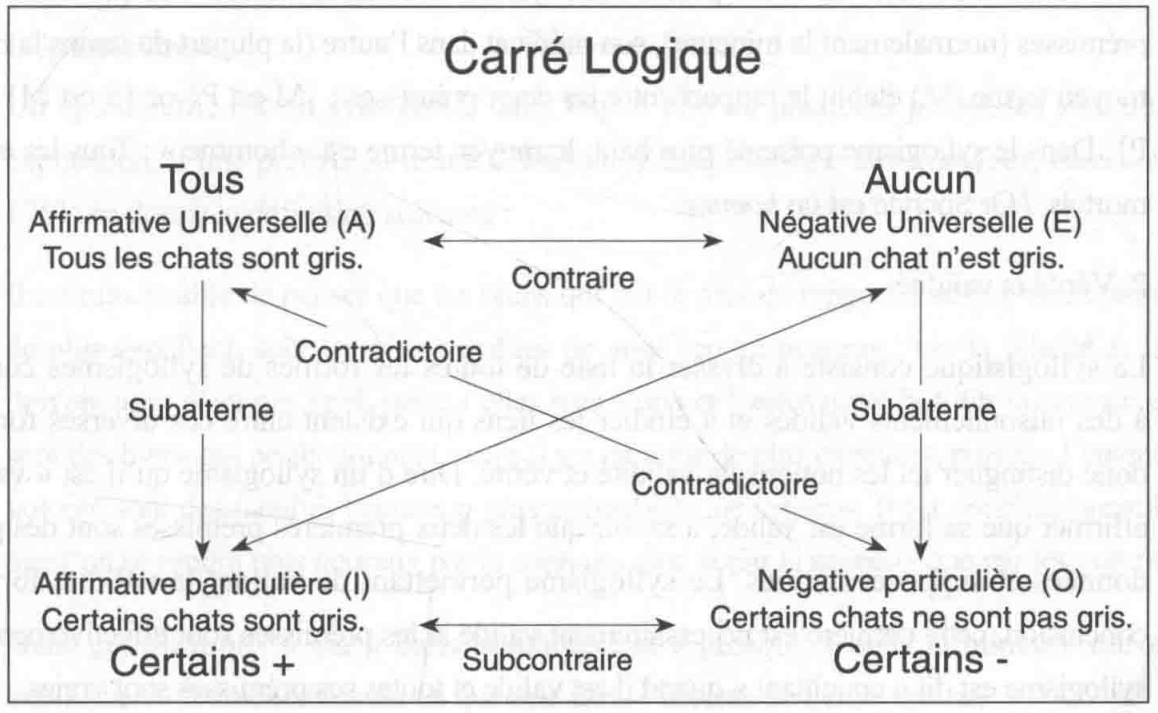
\includegraphics[width=\linewidth]{assets/ch04_square_original.png}\end{center}

\subsection{Les \textit{Premiers Analytiques}}
Les \textit{Premiers Analytiques} constituent le troisième livre de l’\textit{Organon} et la première partie des \textit{Analytiques}. Aristote y développe l’essentiel de sa logique et de la syllogistique, science du syllogisme. Cette dernière constitue la naissance de la logique comme discipline formelle.

\subsubsection*{\textcircled{\scriptsize 1} Le syllogisme}
En logique, le syllogisme est un raisonnement logique mettant en relations trois propositions : deux d’entre elles, appelées « prémisses », conduisent à une « conclusion ». Il s’agit donc d’une inférence déductive. Aristote en donne la définition suivante :

\begin{lecture}{Définition : \textit{Premiers Analytiques} (extrait)}
Le syllogisme est un raisonnement où, certaines choses étant prouvées, une chose autre que celles qui ont été accordées se déduit nécessairement des choses qui ont été accordées.
\end{lecture}

\origpage{104}{090}
Un exemple très connu de syllogisme est :
\begin{itemize}
\item Tous les hommes sont mortels.
\item Socrate est un homme.
\item Donc Socrate est mortel.
\end{itemize}

\minititle{1. Les propositions}
Les syllogismes sont constitués de propositions contenant un sujet (désigné par S) relié par une copule à son prédicat (désigné par P). Pour que le syllogisme soit valide, ces propositions doivent être construites dans un ordre précis : le sujet de la conclusion doit être présent dans une des prémisses (normalement la mineure), son prédicat dans l’autre (la plupart du temps la majeure). Le moyen terme (M) établit le rapport entre les deux prémisses : \{M est P\} or \{S est M\} donc \{S est P\}. Dans le syllogisme présenté plus haut, le moyen terme est « homme » : Tous les hommes sont mortels. / Or Socrate est un \textit{homme}.

\minititle{2. Vérité et validité}
La syllogistique consiste à dresser la liste de toutes les formes de syllogismes correspondant à des raisonnements valides et à étudier les liens qui existent entre ces diverses formes. Il faut donc distinguer ici les notions de validité et vérité. Dire d’un syllogisme qu’il est « valide », c’est affirmer que sa forme est valide, à savoir que les deux premières prémisses sont des propositions données et supposées vraies. Le syllogisme permettant de valider la validité formelle de la conclusion, cette dernière est nécessairement valide si les prémisses sont effectivement vraies.\ednote{概念订正：有效性是论证或推理形式的性质，真值是命题的性质。有效推理保证：若前提全真，则结论必真；仅仅“把前提假定为真”不足以构成有效性的定义。此处结论“nécessairement valide”宜改为“nécessairement vraie”，并明确以前面的推理形式有效为条件。} Un syllogisme est dit « concluant » quand il est valide et toutes ses prémisses sont vraies.

\subsubsection*{\textcircled{\scriptsize 2} L’enthymème}
Dans une argumentation, on peut parfois choisir de ne pas développer entièrement le syllogisme, de façon à éviter la lourdeur des répétitions ou les truismes. Dans ce cas-là, une des prémisses, même la conclusion peut être implicites. Ce type de syllogisme, qui semble n’avoir qu’un argument, est appelé par Aristote « enthymème », c’est-à-dire une inférence déductive dans laquelle le syllogisme est réduit à deux termes.\ednote{按本段关于省略一个前提或结论的说明，应是把明说的命题减少为两个，而不是把三段论的项减少为两个：“deux termes”在这里宜作“deux propositions exprimées”。“une des prémisses, même la conclusion peut être implicites”数的一致亦有问题；可作“une des prémisses, voire la conclusion, peut être implicite”。} Dans sa \textit{Rhétorique}, Aristote définit ainsi l’enthymème :

\begin{lecture}{Définition : \textit{Rhétorique} (extrait)}
Les propositions de l’enthymème sont peu nombreuses, souvent moins nombreuses que celles d’où se tire le syllogisme de la première figure ; en effet, si l’une des prémisses est connue, il n’est même pas besoin de l’énoncer, l’auditeur la supplée. [...] Il ne faut ni prendre le raisonnement de loin ni passer par tous les échelons pour conclure ; le premier procédé manque de clarté par suite de longueur ; l’autre est bavardage, parce qu’il énonce des choses évidentes.
\end{lecture}

\origpage{105}{091}
L’enthymème ci-dessous est tiré de la première méditation des \textit{Méditations physiques} de Descartes.\ednote{书名订正：此处和下面引文标题均误作“Méditations physiques”，应为“Méditations métaphysiques”；本章此前所列书名亦作后者。} La conclusion du syllogisme est implicite. Saurez-vous la deviner ?

\begin{lecture}{Lecture : \textit{Méditations physiques}, Première méditation (extrait)}
Tout ce que j’ai reçu jusqu’à présent pour le plus vrai et le plus assuré, je l’ai appris des sens, ou par les sens : or, j’ai quelquefois éprouvé que ces sens étaient trompeurs, et il est de la prudence de ne se fier jamais entièrement à ceux qui nous ont trompés.
\end{lecture}

\subsubsection*{\textcircled{\scriptsize 3} L’épichérème}
Un épichérème est un syllogisme dans lequel une ou plusieurs prémisses sont suivies d’une explication, d’une preuve ou d’une définition. L’\textit{Encyclopédie des Lumières}, dans son édition de 1751, en donne la définition suivante :

\begin{quote}
Il est raisonnable de penser que les biens qui ont le plus de rapport à ce que notre nature renferme de plus excellent, sont les plus capables de nous rendre heureux ; car la félicité \& la perfection doivent aller d’un pas égal, puisqu’elles sont l’une et l’autre notre but. Or la science et la sagesse sont des biens qui perfectionnent ce qu’il y a en nous de plus excellent, puisque l’entendement et la volonté sont des facultés beaucoup plus estimables que les sens. Il est donc raisonnable de penser que l’on se rendra plus heureux par la connaissance \& par la sagesse, que par les voluptés des sens.
\end{quote}

Dans cet exemple, « car » dans la majeure et « puisque » dans la mineure introduisent des explications. L’épichérème est en quelque sorte l’inverse de l’enthymème.

\subsection{\textit{Isagoge}, de Porphyre}
\textbf{Porphyre de Tyr} (234-310), disciple du philosophe néoplatonicien \textbf{Plotin} (205-270) est l’auteur d’une \textit{Introduction aux Catégories d’Aristote} plus connue sous le titre d’\textit{Isagogè}.

\subsubsection*{\textcircled{\scriptsize 1} Les cinq universaux}
Cinq universaux, appelés aussi « prédicables » ou \textit{quinque voces} (« cinq voix »), constituent le cœur de l’\textit{Isagogè}. Par prédicables (du latin \textit{praedicabilis}, « ce qui peut être dit, ou affirmé »), Porphyre désigne les relations par lesquelles un prédicat peut se rapporter à son sujet. Ce sont :
\begin{itemize}
\item le genre (\textit{genos})
\item l’espèce (\textit{eidos})
\item la différence (\textit{diaphora})
\item le propre (\textit{idion})
\item l’accident (\textit{sumbebekos})
\end{itemize}

\origpage{106}{092}
Les cinq universaux de Porphyre ont été directement inspirés des quatre universaux qu’Aristote distinguait dans ses \textit{Topiques} : genre, espèce, propre et accident. Porphyre y a rajouté la \textit{diaphora}. Pour lui, une bonne définition fait intervenir trois des cinq universaux : le genre, l’espèce et la différence.

\begin{lecture}{Lecture : \textit{Isagoge} (extrait 1)}
Parmi les attributs, les uns ne s’appliquent qu’à un seul être, tels sont les attributs individuels, Socrate par exemple, ou bien tel homme, ou telle chose. D’autres, au contraire, s’appliquent à plusieurs êtres, comme les genres, les espèces, les différences, les propres et les accidents, qui sont communs à plusieurs et non particuliers à un seul individu.

Ainsi, par exemple, le genre c’est animal, l’espèce c’est homme, la différence c’est raisonnable, le propre c’est susceptible de rire, l’accident c’est être blanc, être noir, être assis. Les genres diffèrent donc des attributs qui ne s’appliquent qu’à un seul individu, en ce qu’ils sont au contraire attribués à plusieurs.
\end{lecture}

\subsubsection*{\textcircled{\scriptsize 2} L’arbre de Porphyre}
Dans l’\textit{Isagogè}, Porphyre établit une représentation visuelle et hiérarchisée des dix catégories d’Aristote. Cette hiérarchie, qui a été très largement reprises les manuels médiévaux,\ednote{语法订正：“reprises les manuels”应为“reprise dans les manuels”。下图实际展示的是“实体”属下的逐层划分，并没有展示前文列举的全部十范畴，因此不宜将图本身称作十范畴的层级图。} est connue sous le nom d’\textit{Arbor porphyriana} (« arbre de Porphyre »).
\begin{center}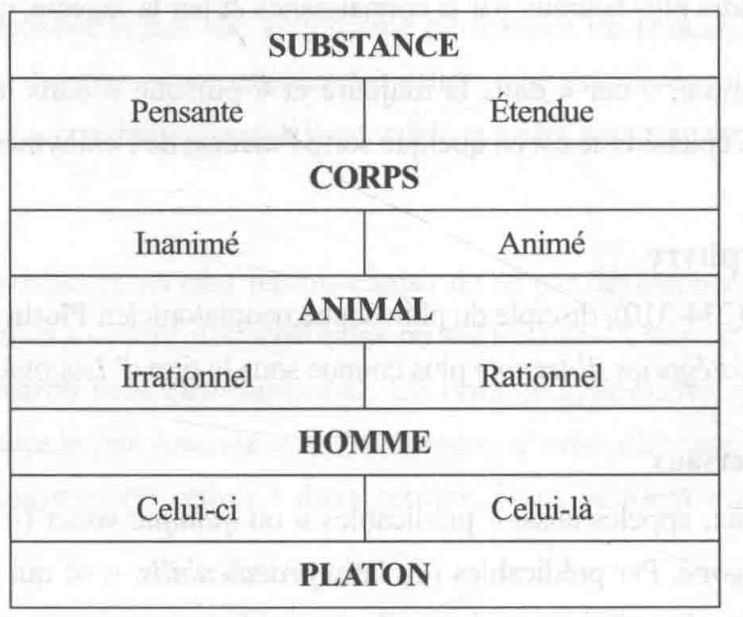
\includegraphics[width=.66\linewidth]{assets/ch04_porphyre_original.png}\end{center}

Pour illustrer la manière dont s’opèrent les divisions génériques, prenons un exemple qui, à partir de la substance (la plus générique) aboutit à l’être humain (le plus spécifique). Le genre « substance » se divise en substance étendue et substance pensante. Ces deux substances se divisent en deux nouveaux genres : « corps » et « esprit ». Le genre « corps » se divise à son tour en « animé » ou « inanimé », qui donnent deux nouveaux genres : « être vivant » et « minéral ». Le genre « être vivant » se divise en « sensible ou insensible », qui donnent à leurs deux nouveaux genres : « animal » et « végétal ». Le genre « animal » se divise en « rationnel » ou « irrationnel »,\origcont{107}{093} qui donnent deux espèces : « humain » et « bête ». Enfin, l’espèce « humain » se divise enfin à son tour en individus : Socrate, Platon, Lionel, etc. L’extrait ci-dessous nous rappelle, si nous en doutions, que l’homme « est bien une espèce de l’animal ».

\subsubsection*{\textcircled{\scriptsize 3} La question des « universaux »}
En guise de conclusion sur la logique aristotélicienne et de transition avec la logique médiévale, je voudrais préciser que dans l’histoire de la philosophie, l’\textit{Isagogè} est célèbre pour avoir lancé un débat sur le statut des « universaux », définis comme « les genres et les espèces » dans l’extrait ci-dessous : existent-ils seulement dans l’esprit, ou aussi par eux-mêmes dans la réalité ? S’ils sont réels, sont-ils des entités physiques ou psychiques ? S’ils sont physiques, ont-ils une existence séparée des corps physiques, ou en font-ils partie ?

\begin{lecture}{Lecture : \textit{Isagoge} (extrait 2)}
Tout d’abord, en ce qui concerne les genres et les espèces, la question est de savoir si ce sont des réalités subsistantes en elles-mêmes ou seulement de simples conceptions de l’esprit, et, en admettant que ce soient des réalités substantielles, s’ils sont corporels ou incorporels, si, enfin, ils sont séparés ou ne subsistent que dans les choses sensibles et d’après elles. J’éviterai d’en parler. C’est là un problème très profond et qui exige une recherche toute différente et plus étendue.
\end{lecture}

« Un problème très profond » ? Porphyre ne croyait pas si bien dire : les questions ci-dessus vont alimenter le plus grand débat logique et métaphysique du Moyen Âge, qui verra s’affronter (violemment parfois) les deux camps des « réalistes » et « nominalistes » jusqu’à la fin du 15\textsuperscript{e} siècle. Ce débat est appelé « Querelle des Universaux ».

\section{Philosophie médiévale : la « querelle des universaux »}
Dans le chapitre précédent, consacré à la grammaire, nous avons déjà évoqué les universaux à travers la notion d’\textit{akriti} que l’on trouve dans le \textit{Grand Commentaire} (\textit{Mahābhāṣya}) de la grammaire de Panini. En Europe, bien des siècles plus tard, cette question des universaux a été à l’origine d’un débat intellectuel majeur qui a traversé tout le Moyen Âge, et même au-delà. Dans la philosophie occidentale, et les universaux (genre, espèce, etc.) qui ont un caractère universel dans le sens où ils peuvent selon Aristote « être dits de plusieurs », c’est-à-dire être conçus comme propres à plusieurs choses singulières différentes.\ednote{原句“Dans la philosophie occidentale, et les universaux ...”结构残缺，可能混入多余的“et”并漏去主句谓语；不在正文中猜补。下段“Les tenants du nominalistes”应为“Les tenants du nominalisme”。同段所否定的是共相作为独立实在的存在，而非“普遍词项”作为词语或概念的存在，后一句的说明也表明了这一点。} La question centrale débattue en métaphysique est alors de savoir si les universaux ont une existence en soi (c’est la thèse du réalisme) ou s’ils ne sont que de simples concepts, de simples mots, produits par l’esprit (thèse du nominalisme). Et s’ils ont une existence réelle, alors comment s’articule-t-elle avec l’existence des particuliers ?

\subsection{Le nominalisme}
Les tenants du nominalistes (Jean Roscelin, Jean Buridan, Guillaume d’Ockham) refusent l’existence des termes universels. Selon eux, il n’existe rien dans le monde réel qui corresponde au terme « animal »
\origcont{108}{094} ou « homme » : il n’existe que des animaux ou des hommes particuliers. Un cheval existe, mais le concept de « chevalinité » ou de « cabalité » n’existe pas. Les universaux ne sont que des concepts abstraits qui viennent \textit{après} (en latin, \textit{post rem}) la chose.

\subsubsection*{\textcircled{\scriptsize 1} Roscelin de Compiègne}
\textbf{Roscelin de Compiègne} (1050-1121), philosophe scolastique français, est considéré comme le fondateur du nominalisme. Sa pensée Roscelin marque un changement important dans la philosophie médiévale :\ednote{句法订正：“Sa pensée Roscelin”混合了两种构句，可作“La pensée de Roscelin”或“Sa pensée”。} il est en effet le premier à avoir soutenu la \textit{sententia vocum}, la doctrine des mots selon laquelle les genres et les espèces sont des \textit{flatus vocis} (« des émissions de voix ») et non des choses. Ainsi, un individu particulier est réel, le mot que l’on emploie pour le désigner désigne quelque chose de réel, mais l’espèce et le genre ne le sont pas.

\subsubsection*{\textcircled{\scriptsize 2} Jean Buridan}
Philosophe français, docteur en scolastique, \textbf{Jean Buridan} (1292-1363) a étudié à l’université de Paris sous la direction du grand philosophe Guillaume d’Ockham.

Impossible de parler de Jean Buridan sans parler du célèbre « âne de Buridan » qui, placé à égale distance entre un seau d’avoine et un seau d’eau, meurt de faim et de soif, faute d’avoir pu faire un choix. À proprement parler, ce cas de figure n’est pas un paradoxe logique, mais plutôt d’un cas de dilemme poussé à l’absurde illustrant ce qu’on appelle le phénomène de « double contrainte ». En réalité, ce « paradoxe » de l’âne, que l’on attribue à Buridan, n’apparaît dans aucune de ses œuvres connues : c’est dans son commentaire du \textit{Expositio in De caelo} (« Traité du ciel ») d’Aristote que Buridan met en scène, non pas un âne, mais un chien confronté au cruel dilemme. Dans \textit{De Caelo} d’Aristote, ce n’est ni un âne, ni un chien, mais un homme, tout simplement, qui doit choisir entre deux nourritures également attirantes :

\begin{lecture}{}
Celui qui, affligé d’une faim et d’une soif très vives, mais également intenses, se trouve à égale distance des aliments et des boissons : lui aussi demeurera nécessairement immobile !
\end{lecture}

\subsubsection*{\textcircled{\scriptsize 3} Guillaume d’Ockham}
Philosophe, logicien et théologien anglais, \textbf{Guillaume d’Ockham} (1285-1347), membre de l’ordre de Saint-François d’Assise, est considéré comme le représentant le plus éminent de l’école nominaliste. Professeur à Oxford, sa doctrine, comme celle de Roscelin, et de son élève Buridan, a été soupçonnée d’hérésie par les autorités ecclésiastiques parce qu’elle remettait en cause bon nombre des postulats de la théologie traditionnelle. On voit parfois dans la philosophie d’Ockham la préfiguration de la science moderne, de l’empirisme anglais ainsi que de la philosophie analytique contemporaine car elle insiste surtout sur les faits et sur le discours rationnel et s’oppose à la spéculation métaphysique. Comme Roscelin, donc, Guillaume d’Ockham a défendu une philosophie nominaliste dans laquelle les concepts universels et abstraits comme par exemple l’homme, l’animal, ne sont que des mots, des représentations dont il récuse le réalisme, c’est-à-dire la réalité substantielle. Pour lui, même si l’utilisation des universaux est nécessaire pour\origcont{109}{095} permettre à la pensée de se constituer, la connaissance véritable s’appuie sur les choses sensibles et singulières, et non abstraites et universelles.

\minititle{1. Un précurseur de la philosophie du langage}
S’appuyant sur Boèce et son commentaire de \textit{De l’interprétation} d’Aristote, Ockham affirme dans sa \textit{Summa totius logicae} (« Somme logique ») publiée en 1323 qu’il y a trois sortes de phrases et de termes : écrites, parlées et conçues. Il considère également les mots comme des signes conventionnels, dont la signification est arbitraire, et qui se rapportent aux idées ou concepts mentaux.

\minititle{2. Le rasoir d’Ockham}
Si Buridan est célèbre pour son âne, Ockham est connu pour son rasoir. Appelé « principe de simplicité », « principe de parcimonie » ou encore « principe d’économie », le « rasoir d’Ockham » est un principe de raisonnement attribué Guillaume d’Ockham qui consiste à ne pas utiliser de nouvelles hypothèses tant que celles déjà énoncées suffisent, et à utiliser autant que possible les hypothèses déjà faites avant d’en introduire de nouvelles. L’idée derrière ce principe est simple : inutile de chercher une explication compliquée, faisant appel à des principes hors du champ de l’expérience (essences des universaux, volonté divine, miracle, etc.), quand une explication simple, à partir de ce que nous connaissons déjà, suffit pour rendre compte d’un phénomène qui se manifeste à nos sens. Ockham rejette donc les concepts aristotéliciens abstraits de « substance », de « cause efficiente », de « puissance », etc. c’est-à-dire tout ce qui, sous prétexte de mieux comprendre la réalité, ne fait que s’obscurcir sous un voile métaphysique. La logique d’Ockham a exercé une grande influence à l’époque moderne sur Gottlob Frege, Bertrand Russell, et Ludwig von Wittgenstein : ils seront tous trois présentés en très détail dans un instant.\ednote{语法订正：“attribué Guillaume d’Ockham”漏去介词，应为“attribué à Guillaume d’Ockham”；“en très détail”应为“en grand détail”或“très en détail”。正文保留原貌。}

\subsection{Le réalisme}
Prenant le contrepied des nominalistes, les réalistes considèrent que les universaux (la blancheur, l’homme, le rouge) ont une existence réelle et que les noms ont une réalité : c’est la thèse « réiste » (du latin \textit{res}, la chose). Selon eux, les individus particuliers (vous, moi, votre voisin, Socrate), partagent une même essence, qui existe. Ils lui sont subordonnés, et ne sont différents dans leurs « accidents ».

Cette doctrine réaliste découle du réalisme des Idées (Essences) de Platon. Selon lui, le monde sensible n’est, en effet, qu’apparence par rapport aux Idées elles-mêmes, objets de la pensée pure, modèles intelligibles de toutes choses, non perçues par les sens, mais néanmoins beaucoup plus réelles et plus vraies que les objets empiriques. Ainsi l’Idée de table, c’est la table idéale, telle que nous la concevons par la pensée, modèle ou paradigme que les tables concrètes imitent et reproduisent. Dans sa \textit{Métaphysique}, Aristote fait la différence entre les propriétés « accidentelles » (occasionnelles), et les propriétés « essentielles » (éternelles). L’accident est ce qui appartient à un être, et qui aurait aussi pu ne pas lui appartenir, puisque sans lien avec son essence (substance) : par exemple, être chinois, ou des cheveux blonds. Pour les réalistes, il n’y a pas une essence relative à Platon et une essence relative à Socrate, mais une seule essence universelle de l’homme, qui existe indépendamment d’eux, et\origcont{110}{096} même les précède. Autrement dit, le concept précède la chose. Ce qui rend Platon différent de Socrate, ce n’est pas une essence différente, mais des accidents dans ce qu’Aristote appelle l’actualisation de l’essence.

\subsubsection*{\textcircled{\scriptsize 1} Guillaume de Champeaux}
Né à Champeaux, près de Melun en région parisienne, \textbf{Guillaume de Champeaux} (1070-1121) est philosophe, logicien et théologien. Après avoir étudié avec \textbf{Anselme de Laon} (1050-1117), il a enseigné dès 1098 la rhétorique, la dialectique et la théologie à l’école de la cathédrale Notre-Dame de Paris où, comme Roscelin, il a été le professeur de Pierre Abélard avant de s’opposer à lui et de lui interdire d’enseigner à Paris en raison de leur divergence sur les universaux. On considère Guillaume de Champeaux comme le fondateur du réalisme radical qui soutient que les universaux existent aussi bien dans l’esprit humain que des objets particuliers. Une même caractéristique se retrouve par essence en même temps tout entière dans chacun des individus du groupe, et donc la diversité ne vient aucunement de l’essence : c’est la multiplicité des « accidents » qui entraîne la variété.

\subsubsection*{\textcircled{\scriptsize 2} La thèse conceptualiste : Pierre Abélard}
Rejetant à la fois les thèses de Roscelin et de Guillaume de Champeaux, essayant de sortir de l’opposition entre la \textit{vox} des nominalistes et la \textit{res} des réalistes, Pierre Abélard a adopté une position intermédiaire : le conceptualisme.

Le conceptualisme de \textbf{Pierre Abélard} (1079-1142) accorde une réalité aux concepts et refuse de les réduire à de simples mots (position du réalisme), mais il ne leur accorde aucune réalité substantielle (position du nominalisme). Le concept, idée générale ou abstraite, est un objet \textit{mental}, qui n’existe que dans l’esprit. Dans l’optique conceptualiste, un concept (par exemple, l’idée de rose, de rouge) est distinct des choses auxquelles il s’applique (une rose rouge concrète), ce qui s’oppose aux théories réalistes. Le concept est aussi distinct des mots (« rose », « rouge ») qui signifient ce concept, ce qui le distingue du nominalisme. Autrement dit, les idées générales n’existent pas de façon absolue. Elles n’existent pas antérieurement aux choses et n’en sont pas non plus l’essence : ce sont des constructions de l’esprit. Pour autant, ce ne sont pas seulement des sons, des noms, ou de pures émissions de « voix », comme le prétend le nominalisme. Elles ont une bien réalité, mais intellectuelle : les universaux sont des constructions mentales, des instruments logiques. Pour Abélard, il n’y a rien d’universel dans la réalité : l’universalité est le fruit d’une opération mentale qui prend en considération les aspects dans lesquels les choses individuelles se regroupent par similitude, en faisant abstraction des aspects différents. L’universel est donc une \textit{vox significativa}, représentation mentale chargée de signification. C’est notre esprit qui opère sur le particulier un travail d’abstraction qui le dépouille de ses particularités pour ne considérer que les éléments communs : les universaux ont donc un fondement objectif dans la réalité.\ednote{排印订正：“Elles ont une bien réalité”应为“Elles ont bien une réalité”。}

\origpage{111}{097}
\section{La période moderne : la rupture épistémologique}
La fin du 19\textsuperscript{e} siècle et le début du 20\textsuperscript{e} siècle ont vu les sciences de la pensée formelle et du langage prendre deux chemins différents. Il s’agit d’une rupture épistémologique, notion forgée par le philosophe français \textbf{Gaston Bachelard} (1884-1962) dans son ouvrage \textit{La Formation de l’esprit scientifique} (1938).

\subsection{Gottlob Frege : naissance de la logique moderne}
Mathématicien et philosophe allemand, \textbf{Gottlob Frege} (1848-1925) est l’un des plus grands logiciens avec Aristote et Ockham. Fondateur de la logique moderne, il a créé une langue artificielle formalisée : l’idéographie qui avait pour but de représenter de manière parfaite la logique mathématique. Le projet d’un langage entièrement formalisé n’était pas nouveau : le grand mathématicien et logicien \textbf{Gottfried Wilhelm Leibniz} (1646-1716) en avait développé un sous le nom de « caractéristique universelle », mais son projet n’avait pas abouti.

\subsubsection*{\textcircled{\scriptsize 1} \textit{Que la science justifie le recours à une idéographie} (1882)}
En 1882, Frege publie dans la revue \textit{Zeitschrift für Philosophie und philosophische Kritik} (« Revue de philosophie critique ») un article intitulé « Que la science justifie le recours à une idéographie ». À travers ce petit texte de seulement quatre pages, il se propose de montrer pour quelles raisons une écriture idéographique formelle est nécessaire dans les sciences abstraites. Frege commence par reconnaître que c’est le langage qui nous permet de conceptualiser, de penser :

\begin{lecture}{}
Sans les signes, nous nous élèverons difficilement à la pensée conceptuelle. [...] Nous avons besoin de signes sensibles pour penser.
\end{lecture}

Puis il précise que bien qu’étant l’instrument de notre pensée, le langage usuel présente des imperfections. D’abord, il n’est pas univoque, et un même mot peut en effet désigner à la fois un concept et un objet particulier : par exemple, dans « Le cheval est un herbivore. », « cheval » apparaît en tant qu’espèce. Dans « Ce cheval est un herbivore. », « cheval » apparaît en tant qu’individu. En outre, notre langage naturel n’est pas régi par des règles logiques. Les différents paradoxes, faux syllogismes et sophismes présentés plus haut sont le fait de propositions grammaticalement correctes mais qui ne reflètent pas les règles de logiques : elles conduisent donc à des erreurs d’interprétation et des raisonnement erronés. Frege en conclut notre langage ne permet pas de donner une expression rigoureuse à nos raisonnements et ne peut non plus exprimer de manière explicite et simple tous les éléments logiques d’une déduction. En outre, si nous essayons de formuler un raisonnement logique dans notre langage usuel, en exprimant toutes les distinctions et déductions, il se révèle bien trop lourd à manier. Ainsi les rapports logiques demeurent-ils toujours tacites. Comme les langues ordinaires pèchent par équivocité des signes, et aussi par le fait qu’elles ne sont pas calquées sur les lois objectives de la pensée mais sur celles de la psychologie humaine, il convient alors de mieux distinguer les deux, grâce à l’invention d’une langue spéciale, calquée sur les exigences logiques :\ednote{语法订正：“des raisonnement”应为“des raisonnements”；“Frege en conclut notre langage”应补“que”，即“Frege en conclut que notre langage”。}

\origpage{112}{098}
\begin{lecture}{}
Les sciences abstraites ont besoin d’un moyen d’expression pour prévenir les erreurs d’interprétation et les fautes de raisonnement.
\end{lecture}

\subsubsection*{\textcircled{\scriptsize 2} \textit{Sens et dénotation} (1892)}
\textit{Sens et dénotation} est un article de Gottlob Frege publié en 1892. Frege y distingue les notions de sens et de dénotation.

\minititle{1. La dénotation}
Selon Frege, la dénotation d’une expression linguistique est la réalité que cette expression désigne à l’aide de cette expression. La dénotation des expressions nominales comme les noms propres et les descriptions définies est un objet du monde ou une chose perceptible, identifiable et individualisable. Avec la dénotation, on se trouve dans le monde extralinguistique.\ednote{范围说明：这里不能把所有指称对象限制为可感知的具体事物。下文原书自己的数学例子“2+2”和“3+1”指向数4，已说明必须容纳抽象对象。此外，“l’étoile du matin”等是名词性表达式，而不是可判真假的完整命题；下段反复用“propositions”称这些例子时，宜改为“expressions”。}

\minititle{2. Le sens}
Frege définit le sens d’une expression comme « le mode de donation » de la dénotation de cette expression. Il faut donc comprendre ici le sens comme une fonction mentale qui, partant d’une expression linguistique, fait le lien entre l’univers du langage et l’univers extralinguistique. Frege nous rappelle que si notre langage usuel était parfait, il serait univoque : « un sens déterminé devrait correspondre à chaque expression ». Mais les langues « vulgaires », comme il les appelle, sont imparfaites. Ainsi, une proposition peut avoir un sens, mais ne pas avoir de dénotation : par exemple, « le corps céleste le plus éloigné de la terre », ou « la suite qui converge le moins rapidement » ne réfèrent à rien d’existant dans l’univers extralinguistique. D’autre part, des propositions de sens différent peuvent partager la même dénotation : « l’étoile du matin » et « l’étoile du soir » réfèrent au même objet : la planète Vénus. De même, « l’auteur de l’Organon » et « le disciple de Platon » réfèrent à Aristote. Dans le domaine des mathématiques, l’expression « 2+2 » a la même dénotation que « 3+1 », mais pas le même sens. Deux concepts distincts peuvent renvoyer à un seul et même objet, mais si le concept se dit d’un objet, il ne se confond pas avec lui.

\minititle{3. L’intension et extension}
La distinction frégéenne entre sens et dénotation est à rapprocher des notions d’intension et extension. En logique aristotélicienne, l’intension est définie comme l’ensemble des prédicats (attributs) qui appartiennent à un concept. L’extension, quant à elle, est l’ensemble des choses du monde auquel l’intension s’applique. Intension et extension sont deux façons de définir un concept ou un objet. Par exemple, la définition en intension de « chat » est : « animal domestique à quatre pattes de la famille des félins ». Sa définition en extension sera : mon chat, le chat de mon voisin, un chat blanc, ce chat sur le canapé, etc.

\origpage{113}{099}
Nous avons vu un peu plus haut avec Frege que ce qu’on appelle des « descriptions définies », comme « le corps céleste le plus éloigné de la terre » ou « la suite qui converge le moins rapidement » ont un sens mais pas de dénotation. Dans le vocabulaire moderne de la logique, on dira qu’elles ont une intension mais pas d’extension, ou encore qu’elles sont une « extension vide ». C’est sur ce point précis que Bertrand Russel va s’opposer à Frege et rejeter la distinction entre connotation et dénotation.\ednote{姓名订正：“Russel”应为“Russell”。概念上，没有指称对象的单称描述与外延为空的谓词须加区分，不能一概视为同一种语义对象。Russell 的方案是在句子层次消去限定描述，不是简单把不存在的对象替换成“空外延”。参见 \ecite{21}。}

\subsection{Bertrand Russell : naissance de la philosophie analytique}
Parfois qualifié de « Voltaire anglais », \textbf{Bertrand Russell} (1872-1970) est considéré comme l’un des plus importants philosophes du 20\textsuperscript{e} siècle. Mathématicien, logicien, épistémologue, homme politique, prix Nobel de littérature en 1950, il est avec Frege l’un des fondateurs de la logique contemporaine. Soutenant l’idée d’une « philosophie scientifique », Russell est aussi le père de la philosophie analytique. S’appuyant sur une analyse logique du langage pour à mettre en évidence les erreurs de raisonnement, il considère que l’on doit utiliser la logique pour clarifier la pensée.\ednote{语法订正：“pour à mettre”应为“pour mettre”。}

\subsubsection*{\textcircled{\scriptsize 1} Le paradoxe de Russell}
Dans ses \textit{Grundgesetze der Arithmetik} (« lois fondamentales de l’arithmétique ») publié en 1893, Frege souhaitait fonder les mathématiques sur des bases purement logiques. Or, au même moment, Russell travaillait exactement au même projet. Dans une lettre de 1902, Russell a exposé à Gottlob Frege ce qui est connu aujourd’hui comme « le paradoxe de Russell », pour lui montrer que ses \textit{Grundgesetze der Arithmetik} contenaient une contradiction interne (antilogie). L’année suivante, Russell a fait paraître ce paradoxe (ainsi que d’autres) dans ses \textit{The Principles of Mathematics}. La même année, le malheureux Frege a été contraint de rajouter au second volume de ses \textit{Grundgesetze der Arithmetik} un appendice où il expose le paradoxe de Russel, et fait précéder son analyse par aveu d’une grande honnêteté :

\begin{lecture}{}
Pour un écrivain scientifique, il est peu d’infortunes pires que de voir l’une des fondations de son travail s’effondrer alors que celui-ci s’achève. C’est dans cette situation inconfortable que m’a mis une lettre de M. Bertrand Russell, alors que le présent volume allait paraître.
\end{lecture}

\minititle{1. Formulation du paradoxe}
Russell s’est posé la question de savoir si « la classe des classes qui ne sont pas membres d’elles-mêmes est (ou n’est pas) membre de « la classe des classes qui ne sont pas membres d’elles-mêmes ». Et c’est ici que surgit le paradoxe : si on répond affirmativement à la question, on est obligé de concéder que la classe en question ne peut en aucun cas être membre d’elle-même puisqu’elle doit posséder la propriété essentielle des classes dont elle est la classe. Mais si l’on répond négativement, on est obligé de concéder que la classe en question ne peut en aucun cas posséder la propriété essentielle des classes de la classe dont elle n’est pas membre, et qu’elle est donc membre d’elle-même. Chaque réponse conduit à son contraire et il y a contradiction.

\origpage{114}{100}
On donne parfois une formulation imagée de ce paradoxe : un bibliothécaire souhaite dresser un catalogue des catalogues de sa bibliothèque. Le catalogue qui ne se mentionne pas lui-même est appelé « hétéro-catalogue », et le catalogue qui se mentionne lui-même (autoréférentiel) est appelé « auto-catalogue ». Si le bibliothécaire dresse le catalogue des hétéro-catalogues, alors son catalogue qui ne se mentionne pas lui-même doit être inscrit dans le catalogue des hétéro-catalogues. Mais dès qu’on l’y inscrit, il devient un auto-catalogue et doit donc être enlevé de la liste. Mais si on le retire de la liste, il redevient un hétéro-catalogue et doit être réinscrit dans la liste, ainsi de suite.

\minititle{2. La théorie des types}
La solution proposée par Russell est la suivante : tout ce qui contient le tout d’une collection ne peut en aucun cas être membre de cette collection. Ce principe interdit donc la possibilité pour un catalogue ou un ensemble de se mentionner lui-même. Pour résoudre les contradictions de ses paradoxe « autoréférentiels », comme celui du menteur ou du barbier, Russell a développé en 1908 une théorie des types (dite « ramifiée », par rapport au type « simples » de 1903), qui postule qu’à un ensemble ne peuvent appartenir que des objets, qui peuvent être des ensembles, mais qui sont de types strictement inférieurs au type de l’ensemble initial, de sorte qu’on ne peut tout simplement plus écrire le prédicat d’auto-appartenance. La théorie des types ramifiée a l’avantage d’éliminer les antinomies à leur racine, puisqu’elle empêche leur écriture : en effet, écrire $C\in C$, c’est écrire une expression dépourvue de sens, puisque les classes désignées par C ne sont pas de même type. De même pour le menteur : ses mensonges (discours), on l’a vu, sont d’un ordre différent de son énoncé « je mens » (discours sur le discours).

\subsubsection*{\textcircled{\scriptsize 2} \textit{On denoting} (1905)}
En 1905, en réponse à l’article \textit{Sens et dénotation} de Frege, Russell a développé dans \textit{On denoting} (1905) sa théorie des « descriptions finies »,\ednote{术语订正：“descriptions finies”应为“descriptions définies”（限定描述），不是“有限描述”。} qu’il considérait d’ailleurs comme sa contribution la plus importante à la logique. Dans les premières lignes de cet essai, Russell distingue trois espèces d’expressions référentielles :
\begin{itemize}
\item Les expressions référentielles qui ne se réfèrent à rien. Par exemple, « l’actuel roi de France ». On pourrait ajouter l’exemple de Frege, « l’étoile la plus éloignée de la Terre ». Ce sont des descriptions vides.
\item Les expressions référentielles qui ont une dénotation ambiguë. Par exemple, : « un homme ». Ce sont les descriptions indéfinies. Dès 1903, dans ses \textit{Principles of Mathematics} écrivait à leur sujet :
\end{itemize}

\begin{lecture}{}
Si nous disons « j’ai rencontré un homme », la proposition ne se réfère pas au concept « homme », mais bien à l’homme réel dénoté par ce concept. Ce que j’ai rencontré en effet est un homme réel « avec un tailleur et un compte en banque » et non pas un concept « qui habite dans les limbes obscurs des livres de logique et ne se promène pas en rue.
\end{lecture}

\origpage{115}{101}
\begin{itemize}
\item Les expressions référentielles qui se réfèrent à un objet défini. Par exemple, « l’actuelle reine d’Angleterre ». Ce sont les descriptions définies. Pour Russell les descriptions définies ne \textit{nomment} pas un objet, mais \textit{affirment} qu’il existe un objet qui satisfait cette description. C’est ce soupçon sur la structure grammaticale des énoncés du langage ordinaire qui a poussé Russell à étudier la possibilité d’une traduction de ce langage usuel en un langage idéal, celui de la logique. Ce point est essentiel dans la naissance de la philosophie analytique.
\end{itemize}

\minititle{1. « Le roi de France est chauve. »}
Russell estimait que la valeur d’une théorie logique doit être prouvée par sa capacité à résoudre des énigmes (« \textit{A logical theory may be tested by its capacity for dealing with puzzles} »), et il a lui-même formulé quelques énigmes pour tester sa théorie et pour illustrer les difficultés que l’on rencontre lorsque l’on veut s’exprimer clairement au moyen de notre langage ordinaire. « L’actuel roi de France est chauve. » est la plus célèbre de ces « énigmes ». En application de la loi du tiers-exclu :
\begin{itemize}
\item soit la proposition « l’actuel Roi de France est chauve » (a) est vraie,
\item soit la proposition « l’actuel Roi de France est non chauve » (b) est vraie.
\end{itemize}
Or, si nous procédons à la définition en extension du prédicat « chauve », nous ne trouvons pas « l’actuel Roi de France », puisqu’actuellement, il n’y a pas de roi en France, et que c’était déjà le cas en 1905 lorsque Russell a publié \textit{On denoting}. Puisqu’aucun objet ne possède les deux propriétés « est actuellement roi de France » et « est chauve », alors, et contrairement à ce que nous avons dit plus haut :
\begin{itemize}
\item « l’actuel Roi de France est chauve » est fausse.
\item « l’actuel Roi de France n’est pas chauve », est fausse aussi.
\end{itemize}

\minititle{2. La résolution de l’énigme}
Selon Russell, seule une analyse logique correcte de cette proposition peut résoudre l’énigme. Pour retrouver sa forme logique sous-jacente, il faut la démembrer et transformer la description définie en description indéfinie. Ainsi, la proposition « Le roi de France est chauve. », est « traduite » en termes logiques en trois étapes, comme suit :
\begin{itemize}
\item Clause ontologique : il existe un X qui est roi de France.
\item Clause d’unicité : il n’y a qu’un seul X qui soit tel.
\item Assertion : X est chauve.
\end{itemize}
L’article défini disparaît ainsi de la description définie. Cette analyse étant faite, il est facile de voir que cette proposition est fausse, puisque son premier terme est faux. Le principe du tiers exclu est ainsi sauvé, puisqu’il n’est pas question de dire que l’actuel roi de France n’est « ni chauve ni non-chauve », mais que l’actuel roi de France n’existe pas.\ednote{关键补正：必须区别句内否定和句外否定。令 $P$ 为“存在唯一法国国王且他秃头”，句外否定 $\neg P$ 在不存在法国国王时为真；而“存在唯一法国国王且他不秃头”仍为假。后二者不是 $P$ 与 $\neg P$，两者均假不违反排中律。Russell 原文明确区别限定描述的 primary／secondary occurrence。参见 \ecite{21}。} Pour Frege, la définition finie « le\origcont{116}{102} roi de France » a un sens, mais est dépourvue de dénotation. Russell montre que cet énoncé a un sens, mais est faux. Selon lui, toutes les descriptions contenues dans les propositions du langage ordinaire doivent être ainsi démembrées en fonctions propositionnelles. C’est est la thèse qu’il défend dans ses \textit{Principia Mathematica} :\ednote{术语、排印订正：“la définition finie”在此应为“la description définie”；“C’est est”重复，应为“C’est”。注意限定描述“le roi de France”本身不是命题；上句“cet énoncé ... est faux”须理解为完整的秃头断言，而不是单独的名词短语。}

\begin{lecture}{}
Si le sujet grammatical d’une proposition peut être supposé ne pas exister sans rendre la proposition dépourvue de sens, il est évident que le sujet grammatical n’est pas un nom propre et que, donc, dans tous les cas, la proposition doit pouvoir être analysée de telle manière que ce qui en était le sujet grammatical ait disparu. Donc, quand nous disons « le carré rond n’existe pas », nous pouvons lui substituer : « Il est faux qu’il y ait un objet X qui soit à la fois rond et carré. »
\end{lecture}

À l’époque moderne, cette question de la calvitie du roi de France a continué d’intéresser les linguistes contemporains, parmi lesquels le français Oswald Ducrot.

\subsubsection*{\textcircled{\scriptsize 3} Russell et Oswald Ducrot : Posé, présupposé et sous-entendu}
\textbf{Oswald Ducrot} (1930-) s’est beaucoup intéressé dans ses travaux à la question de l’énonciation, c’est-à-dire ce que l’on dit lorsque l’on parle. Le titre de certains de ses ouvrages l’indique d’ailleurs clairement : \textit{La Preuve et le dire} (1973), \textit{Le Dire et le Dit} (1980), \textit{Dire et ne pas dire} (1998). Dans un acte d’énonciation, Ducrot distingue le présupposé, le posé, et le sous-entendu, et note qu’alors que l’on s’engage avec le présupposé et le posé, il n’en va pas de même avec le sous-entendu. Ce dernier est en effet toujours niable. C’est ce qu’illustre le petit dialogue ci-dessous, entre un mari essayant maladroitement de faire un compliment à sa femme :

\begin{quote}
Mari : Chérie, je te trouve encore très belle \textit{pour ton âge}.

Femme : Quoi ? Tu veux dire que je suis vieille ???

Mari : Mais ce n’est pas du tout ce que j’ai dit !
\end{quote}

Ce qui distingue à présent le posé du présupposé est que seul le posé tombe sous le coup de la négation. Ainsi, dans le célèbre exemple de Russell, « Le roi de France est chauve. », il est \textit{présupposé} qu’il existe un roi de France et il est \textit{posé} qu’il est chauve. C’est la raison pour laquelle la négation de « Le roi de France est chauve. », c’est-à-dire « le roi de France n’est pas chauve. », continue de nous engager quant à l’existence du présupposé (il existe un roi de France), même si elle nie le posé, à savoir la calvitie du roi.\ednote{理论层次说明：这里已经转入预设分析，不能把它与前面 Russell 把存在和唯一性纳入断言真值条件的分析等同。普通否定下仍承诺某前提，是预设分析的诊断；Russell 的句外否定则可一并否定存在条件。参见 \ecite{21}。}

Avant de quitter Russell, je vous propose de le faire dialoguer à travers le temps et l’espace avec un logicien bien connu en Chine, Gongsun Long. Nous verrons que la logique occidentale moderne permet d’éclairer les paradoxes des sophistes chinois.

\origpage{117}{103}
\subsubsection*{\textcircled{\scriptsize 4} Russell et Gongsun Long : 白马非马}
Durant la période des Royaumes combattants, l’« École des Noms » (名家) regroupait des sophistes (辩者) connus pour leur art de la controverse et leurs paradoxes. \textbf{Gongsun Long} (325-250 avant J.-C.) est l’un d’entre eux. Parmi les six chapitres qui composent le recueil portant son nom (« \textit{Gongsun Longzi} »), le deuxième est entièrement consacré à son discours le plus célèbre \textit{Sur le cheval blanc} :

\begin{lecture}{Lecture : \textit{Sur le cheval blanc} (extrait)}
Un cheval blanc n’est pas cheval [...] Car si vous cherchez un cheval, on peut vous amener indifféremment un cheval jaune ou noir ; mais si vous cherchez un cheval blanc, on ne peut vous fournir ni un cheval jaune ni un cheval noir [...] C’est pourquoi, bien que le cheval jaune et le cheval noir restent identiques, ils ne peuvent correspondre qu’à « cheval » et non à « cheval blanc ». Il est donc évident que cheval blanc n’est pas « cheval ».
\end{lecture}

Ce paradoxe présente une similitude avec les paradoxes présentés plus haut en ce sens qu’il montre que la logique pure peut conduire à des conclusions assez inattendues. Si, pour Gongsun Long, il faut « rectifier les noms », ce n’est pas pour des raisons morales ou politiques, comme chez Confucius, mais pour créer un ordre logique : tout est différent et il faut donner à chaque chose son nom correct. Je reproduis ci-dessous le texte original du 《白马篇》 :

\begin{lecture}{Lecture : 《白马篇》}
\normalfont
“白马非马，可乎？”曰：“可。”

曰：“何哉？”曰：“马者，所以命形也。白者，所以命色也。命色者，非命形也，故曰白马非马。”

曰：“有白马，不可谓无马也。不可谓无马者，非马也？有白马为有马，白之非马，何也？”

曰：“求马，黄、黑马皆可致。求白马，黄、黑马不可致。使白马乃马也，是所求一也，所求一者，白者不异马也。所求不异，如黄、黑马有可有不可，何也？可与不可其相非明。故黄、黑马一也，而可以应有马，而不可以应有白马，是白马之非马审矣。”

曰：“以马之有色为非马，天下非有无色之马也。天下无马，可乎？”

曰：“马固有色，故有白马。使马无色，有马如已耳，安取白马？故白者非马也。白马者，马与白也；马与白马也，故曰：白马非马也。”

曰：“马未与白为马，白未与马为白。合马与白，复名白马，是相与以不相与为名，未可。故曰：白马非马，未可。”

曰：“以有白马为有马，谓有白马为有黄马，可乎？”曰：“未可。”曰：“以有马为异有黄马，是异黄马于马也。异黄马于马，是以黄马为非马。以黄马为非马，而以白马为有马；此飞者入池，而棺椁异处；此天下之悖言乱辞也。”

曰：“有白马，不可谓无马者，离白之谓也。是离者有白马不可谓有马也。故所以为有马者，独以马\origcont{118}{104}为有马耳，非有白马为有马。故其为有马也，不可以谓马马也。”

曰：“白者不定所白，忘之而可也。白马者，言定所白也。定所白者，非白也。马者无去取于色，故黄、黑皆所以应。白马者，有去取于色，黄、黑马皆所以色去，故唯白马独可以应耳。无去者非有去也。故曰：白马非马。”
\end{lecture}

Pour Gottlob Frege et Bertrand Russell, le langage naturel doit être reformulé dans un langage formel, rigoureux et dénué d’ambiguïté. Russell, par exemple, pense que la copule « est » peut être analysée de trois manières distinctes, exprimant chacune trois idées différentes :
\begin{itemize}
\item la prédication (propriété) : « Le chat est endormi. » (x a la propriété P, soit P(x))
\item l’existence : « Il est un chat. » (il y a un x, soit : $\exists(x)$)
\item l’identité : « Trois est la moitié de six. » (x est identique à y, soit x=y)\ednote{形式记号订正：单写“$\exists(x)$”缺少量词后的公式，不能表示“有一只猫”。令 $C(x)$ 表示“$x$ 是猫”，应写 $\exists x\,C(x)$。下文把个体与种类的不等同解释为“外延不等于内涵”也混淆了层次：个体不是外延集合，种类也不自动等于内涵。应分别说明个体的归属、集合的同一和表达式的意义。}
\end{itemize}

En chinois l’expression 白马非马 (« un cheval blanc n’est pas un cheval ») joue sur l’ambiguïté de 非. Si, comme le recommande Russel, nous traduisons le paradoxe en langue formelle (X 非 Y), où X est cheval blanc et Y est cheval, alors la proposition (X 非 Y) peut signifier :
\begin{itemize}
\item X \textit{n’est pas un membre de l’ensemble} Y, ce qui est faux : un cheval blanc (X) appartient à l’espèce « cheval » (Y). Si nous faisons une définition en extension de « cheval », nous trouverons des chevaux blancs ainsi que des chevaux noirs, marrons, etc.
\item X \textit{n’est pas identique à} Y, ce qui est vrai : un cheval individuel n’est pas identique à l’espèce cheval à laquelle il appartient. Pour reprendre la terminologie de Frege, l’extension (« un cheval blanc ») n’est pas identique à l’intension (le cheval, espèce animale).
\end{itemize}
Par ailleurs, on peut aussi argumenter qu’un cheval blanc possède deux attributs (couleur et forme) alors que l’espèce cheval n’en possède qu’un seul (la forme). Pour la première fois dans la philosophie chinoise, Gongsun Long sépare la nature de chaque espèce de sa réalité concrète et conçoit des concepts universels. Dans son \textit{Histoire de la philosophie chinoise}, \textbf{Feng Youlan} (1895-1990) a donné une explication de ce paradoxe basée sur les oppositions abstrait-concret et universel/particulier :

\begin{lecture}{}
À strictement parler, les noms se divisent entre noms abstraits et ce qui sont concrets. Les mots abstraits se rapportent à l’universel, les mots concrets, au particulier. Le particulier est la dénotation, et l’universel est la connotation du terme. Dans les langues occidentales flexionnelles, il n’est pas difficile de distinguer le particulier (« blanc » or « cheval ») de l’abstrait (« blancheur » or « chevalinité »). Mais en chinois, en raison de l’absence de flexion, on ne peut pas distinguer le particulier de l’abstrait en se basant sur la morphologie des mots. Ainsi, en chinois, le mot désignant un cheval particulier et le concept universel de « chevalinité » s’écrivent et se prononcent de la même façon.
\end{lecture}

\origpage{119}{105}
\subsubsection*{\textcircled{\scriptsize 5} Russell et Zhuangzi : 鱼之乐}
Le célèbre \textit{Bonheur des poissons} de Zhuangzi, bien connu en Chine, nous permet d’apporter une autre illustration à l’analyse de la copule chez Russell.

\begin{lecture}{Lecture : 《鱼之乐》，庄子}
\normalfont
庄子与惠子游于濠梁之上。庄子曰：“鯈鱼出游从容，是鱼之乐也。”

惠子曰：“子非鱼，安知鱼之乐？”

庄子曰：“子非我，安知我不知鱼之乐？”

惠子曰：“我非子，固不知子矣；子固非鱼也，子之不知鱼之乐，全矣。”

庄子曰：“请循其本。子曰‘汝安知鱼之乐’云者，既已知吾知之而问我，我知之濠上也。”
\end{lecture}

Dans le texte ci-dessus, l’analyse de la copule à la forme négative 非 selon la méthode de Russell montre qu’elle exprime deux idées différentes :
\begin{itemize}
\item 子非鱼 : il s’agit du « est » d’existence, à la forme négative
\item 子非我 : il s’agit du « est » d’identité, à la forme négative.\ednote{概念订正：“子非鱼”是否定述谓（你不具有“鱼”的类别属性），不是否定存在。令 $F(x)$ 为“$x$ 是鱼”、$z$ 指“子”，可写 $\neg F(z)$；它既不表示“你不存在”，也不表示“鱼不存在”。“子非我”则可以作个体不相同 $z\ne w$ 的分析。}
\end{itemize}

Quittons la Chine ancienne et revenons en Europe à l’époque moderne. En 1911, Russell va faire la connaissance du jeune philosophe autrichien Ludwig von Wittgenstein. Ce sera, selon ses propres mots, l’une des rencontres les plus déterminantes de son existence philosophique : « \textit{Wittgenstein was one of the most exciting intellectual adventures of my life.} »

\subsection{Ludwig von Wittgenstein : les limites du langage}
\textbf{Ludwig von Wittgenstein} (1889-1951) est un philosophe autrichien naturalisé britannique qui a apporté des contributions décisives en logique, en théorie des fondements des mathématiques et en philosophie du langage. Il n’a publié de son vivant qu’une œuvre majeure : le \textit{Tractatus logico-philosophicus} (1921). Avec ses \textit{Investigations philosophiques}, publiées à titre posthume en 1956,\ednote{年份订正：《哲学研究》首次以德英对照本于1953年身后出版，非1956年；本章原书第109页也明确写作1953，与此处自相矛盾。此处可据同章后文订为1953。} le \textit{Tractatus} est la pièce majeure de la philosophie de Wittgenstein. Considéré comme un des livres de philosophie les plus importants du 20\textsuperscript{e} siècle, ce petit ouvrage d’environ 70 pages a une influence majeure sur la philosophie analytique et le positivisme logique. Dans cette œuvre influencée à la fois par Frege et Russell, Wittgenstein montre les limites du langage et de la faculté de connaître de l’homme, d’où le célèbre aphorisme : « Les limites de mon langage signifient les limites de mon propre monde. »

\subsubsection*{\textcircled{\scriptsize 1} La \textit{Tractatus logico-philosophicus}}
\minititle{1. L’atomisme logique}
Le concept d’atomisme logique, apparu pour la première fois dans \textit{La philosophie de l’atomisme logique} (1989) de Russell, est un héritage des travaux de Gottlob Frege au cours du 19\textsuperscript{e} siècle. Pour ce dernier, la vérité des propositions est fonction des éléments qui constituent cette proposition.\ednote{排印订正：小标题“La Tractatus”应为“Le Tractatus”。书目与年代须区分：这里的1989至多可指后出的版本，不能作为 Russell 最初提出这些思想的年份——原书前页已列其卒年为1970；且本段把它说成1921年《逻辑哲学论》的思想来源。未据此猜改具体初刊年份。}

\origpage{120}{106}
En analysant ses éléments, il est possible de déterminer la valeur de vérité de n’importe quelle proposition. Cet atomisme logique a ultérieurement reçu deux versions différentes chez Russell et son élève Wittgenstein. La thèse défendue par Russell est que ces éléments ultimes sont à la fois des particuliers, c’est-à-dire des sons, des images, des sensations ponctuelles, et des universaux, qui sont les prédicats et les relations de ces particuliers. Les particuliers et les prédicats constituent les atomes de notre connaissance, les constituants primitifs par lesquels nous saisissons le monde et à partir desquels notre connaissance est élaborée. Bien qu’influencé par son professeur, Wittgenstein propose dans le \textit{Tractatus} une théorie atomiste logique sensiblement différente de Russell. S’il affirme comme son professeur que « le monde se décompose en faits », il soutient que ce sont les faits (et non les objets) qui sont les atomes logiques du réel : « Le monde est la totalité des faits, non des choses. » Pour lui, le monde n’est pas un ensemble de choses (arbres, personnes, villes, manuels de linguistique, etc.), mais de faits, comme « Jules aime Julie ».

\minititle{2. Le fait et l’objet}
Bien qu’étant l’unité de base pour Wittgenstein, le fait est lui-même composé d’objets. Wittgenstein distingue deux types d’objet : les particuliers, et les propriétés et relations. Par exemple « Socrate » est un particulier, « ... est philosophe » est une propriété. Le fait « Lionel est professeur » se compose donc de deux objets : un particulier et une propriété. Dans le fait « Jules aime Julie » on a deux particuliers et une relation (aimer), soit trois objets. Les propositions représentent les faits, l’objet est ce à quoi renvoie le nom. Le rôle de l’objet est crucial pour la détermination du sens : une proposition dont les noms ne renvoient pas à des objets est considérée par Wittgenstein comme une pseudo-proposition qui n’a pas de sens. Ce n’est que théoriquement que « le nom signifie l’objet ». Comme nous le verrons un peu plus bas, la signification d’un nom est en fait l’usage de ce nom, les propositions dans lesquelles il peut se trouver. D’où le célèbre aphorisme de Wittgenstein :

\begin{lecture}{}
Si un signe n’a pas d’usage, il n’a pas de signification.\ednote{语境说明：这句话对应《逻辑哲学论》3.328，附近3.326—3.327讨论符号的有意义使用和逻辑句法使用。因此不能仅据此把早期著作直接等同于后文晚期的“意义即使用”分析。参见 \ecite{19}。}
\end{lecture}

\minititle{3. Le sens}
Le \textit{Tractatus} est un ouvrage sur la délimitation du sens : il a pour objet de séparer ce qui peut être dit et ce qui ne peut pas l’être. Tout ne peut en effet être dit de façon sensée : il y a pour Wittgenstein une limite à l’expression des pensées, et toutes les pensées ne sont pas exprimables. L’ouvrage vise donc à établir les critères qui font qu’un discours a un sens, à déterminer ce qu’on peut dire et ce qu’il faut taire. Le verdict de Wittgenstein est clair : essayer d’exprimer l’indicible dans la langue n’amène qu’à un discours insensé. Cette démarcation n’est cependant pas une dévalorisation de l’indicible, dont Wittgenstein reconnaît l’importance, mais c’est en reconnaissant l’indicible comme tel qu’on « le met à sa place ». Il faut le comprendre comme tel et ne pas tenter de le communiquer dans la langue usuelle. Cette idée centrale est exprimée dans l’avant-propos du livre :

\origpage{121}{107}
\begin{lecture}{}
On pourra résumer en quelque sorte tout le sens du livre en ces termes : tout ce qui peut être dit peut être dit clairement, et sur ce dont on ne peut parler, il faut garder le silence.
\end{lecture}

\minititle{4. Les différents types de propositions}
En cherchant à déterminer les limites de ce qui peut se dire de façon sensée, Wittgenstein a différencié les propositions sensées de celles qui ne le sont pas. Il a distingué ainsi trois types d’énoncés (ou propositions) :
\begin{itemize}
\item les propositions sensées ou pourvues de sens
\item les propositions hors du sens, ou vides de sens
\item les propositions insensées, ou dépourvues de sens
\end{itemize}

\minititle{1) Les propositions pourvues de sens}
Cette première catégorie inclut les propositions proprement dites. Pour Wittgenstein, et selon le principe de l’atomisme vu plus haut, une expression possède un sens si ses composants possèdent une dénotation : « Tout jugement sur des complexes peut s’analyser en un jugement sur leurs constituants. » Inversement, toute expression dont les termes ne réfèrent pas à rien de réel se trouvera donc exclue du sens. Autre critère : les propositions sensées sont celles qui sont vérifiables. Pour qu’un énoncé ait un sens, il faut qu’il porte sur un fait empirique observable. S’il n’est pas vérifiable à l’aide de l’expérience, alors c’est soit de la pseudo-science, soit de la métaphysique, dans tous les cas une « pseudo-propositions ». Ainsi une proposition affirmant « il y a un Dieu » n’est ni vraie, ni fausse, mais tout simplement dépourvue de signification, car invérifiable. Les deux catégories suivantes comprennent les « pseudo-propositions » que nous venons d’évoquer.\ednote{几处须分开：（1）“ne réfèrent pas à rien de réel”按上下文应为“ne réfèrent à rien de réel”；“une pseudo-propositions”应为单数。（2）将意义条件直接概括成经验可验证性，把后述证实论读进了《逻辑哲学论》；4.024区分理解命题和知道命题为真。（3）不能把“无内容”与“胡说”并为一类；4.461—4.4611明确说重言式与矛盾式虽无实质内容，却不是无意义的胡说。参见 \ecite{19}。}

\minititle{2) Les propositions vides de sens}
Les propositions vides de sens (hors du sens) sont les propositions formelles de la logique et des mathématiques. Comparables aux jugements \textit{a priori} (analytiques) de Kant, elles ne portent pas sur le réel, mais expriment la forme de notre pensée. Ces propositions n’ont aucun contenu et ne prétendent pas donner d’information. La proposition « $2+2=4$ » ne dit rien sur ce qui existe de réel : c’est une la tautologie de forme « A = A ». De même, « un carré a quatre angles droits » n’est pas plus informatif que « A = A », puisque la définition du carré (« a quatre angles droits ») est incluse dans son concept. De façon plus générale, les formules de la logique et des mathématiques incluent le prédicat dans leur concept : on n’obtient donc de prédicat supplémentaire ou d’affirmation sur le réel, contrairement aux énoncés des sciences empiriques. Si Wittgenstein les exclut du domaine du sens, ces propositions vides de sens ne posent cependant de problèmes car, répétons-le, elles n’ont aucune prétention informative. Il en va différemment des propositions dépourvues de sens.\ednote{此处再把 Kant 的“先天”与“分析”当作同义词是不正确的：Kant 明确讨论先天综合判断，并把纯数学判断列入其中，参见 \ecite{18}，导论V。文字上“une la tautologie”多出冠词；“on n’obtient donc de prédicat”及“ne posent cependant de problèmes”均漏“pas”。此外，四个直角并不足以定义正方形，也适用于非正方形的矩形。}

\origpage{122}{108}
\minititle{\textit{3) Les propositions dépourvues de sens}}
Ce que Wittgenstein appelle « non-sens » recouvre un grand nombre de propositions hétéroclites comprenant les propositions de la métaphysique, de la fiction, de l’éthique ou encore de l’esthétique. Dans le « \textit{Tractatus} », Wittgenstein prend l’exemple suivant : « Ulysse fut déposé sur le sol d’Ithaque dans un profond sommeil. » Cette proposition n’a aucun sens, puisque « Ulysse », personnage de fiction, n’a pas de dénotation.\ednote{引文归属待核：本次在所核对的《逻辑哲学论》德英全文中检索 Ulysses／Odysseus，未找到这一例句。暂保留原文，不把这段转述当作已经确证的该书原话；“没有指称”也不应未经论证就与“没有意义”直接画等号。参见 \ecite{19}。}

La distinction entre dicible et indicible prend ici toute son importance. Les énoncés « dépourvus de sens » sont ceux qui croient dire quelque chose sur le réel, alors même qu’ils ne le font pas, et surtout qu’ils ne le peuvent pas. Pour autant, ce n’est pas parce qu’une proposition est insensée que ce dont elle tente de parler est sans importance. Au contraire, ce dont tentent de parler certaines pseudo-propositions est crucial : l’éthique et l’esthétique sont valorisées par Wittgenstein, qui les rapproche de la logique. Pour lui, l’éthique et l’esthétique sont, comme la logique, les conditions du monde : pas plus qu’on ne peut concevoir un monde sans logique, on ne peut concevoir un monde sans éthique et esthétique. En cela éthique et esthétique sont « transcendantales ». L’erreur réside uniquement dans la tentative de les exprimer dans la langue naturelle, mais le fait qu’on ne puisse en parler ne leur enlève donc aucune importance.

Si éthique et esthétique sont donc valorisées, le \textit{Tractatus} est souvent mentionné pour son aspect résolument antimétaphysique. Wittgenstein y critique en effet une métaphysique absurde qui ne peut pas remplir les conditions du sens puisqu’utilisant des termes sans dénotation : « le premier principe », « absolu », « essence », « premier moteur », « infini », etc... Elle utilise en outre des mots courants non adaptés à leur nouveau contexte d’usage, tombant ainsi dans les pièges du langage ordinaire qui ne correspond pas à la structure réelle de la pensée. En s’attachant à la grammaire naturelle, la métaphysique ne voit pas la « grammaire logique » des mots.

\minititle{5. La philosophie comme « critique du langage »}
Pour Wittgenstein philosophie et science ne se distinguent pas par leur méthode mais par leur objet. La science produit des descriptions vraies du monde, elle a pour objet le réel. La philosophie n’a pas pour objet le réel : elle ne parle pas du monde, et ne peut pas le faire. Il n’y a donc pas de propositions « philo sophiques » comme il peut y avoir des propositions « scientifiques ». Contrairement à Russell, Wittgenstein refuse également l’idée d’un méta-langage : les énoncés de la philosophie ne sont pas des méta-énoncés, mais des pseudo-propositions. Wittgenstein conçoit la philosophie comme une activité de clarification logique des pensées, qui dévoile la forme logique des énoncés derrière leur expression en langue naturelle. En ce sens, elle est une critique du langage.\ednote{排印订正：“philo sophiques”中间的空格应删，作“philosophiques”。}

\subsubsection*{\textcircled{\scriptsize 2} La « seconde philosophie » de Wittgenstein}
Au cours de discussions avec le logicien \textbf{Frank Ramsey} et les savants du Cercle de Vienne\origcont{123}{109} (qui seront présentés un peu plus bas), Wittgenstein a commencé à s’interroger et à envisager la possibilité que son travail ait pu comporter des erreurs. Il est alors revenu sur quatre thèses du \textit{Tractatus} :
\begin{itemize}
\item l’atomisme logique : les énoncés élémentaires sont indépendants les uns les autres
\item l’extensionalité : la valeur de vérité d’une proposition dépend de la valeur de vérité des propositions qui la composent
\item le langage a pour rôle de représenter le monde
\item la logique est le seul langage parfait
\end{itemize}
C’est cette autocritique sévère et rare dans l’histoire de la philosophie qui a marqué le début de sa seconde carrière de philosophe. Il a développé alors une nouvelle méthode philosophique et proposé une nouvelle manière d’appréhender le langage, avec notamment deux nouveaux principes :
\begin{itemize}
\item La philosophie ne doit pas s’occuper d’un langage idéal mais doit s’intéresser au langage ordinaire.
\item La signification du nom n’est pas l’objet. La signification réside dans l’usage sémantique.
\end{itemize}

\minititle{1. La philosophie linguistique : retour au langage ordinaire}
\textit{Investigations philosophiques} (1953) est un ouvrage posthume de Wittgenstein traitant principalement de sémantique et de la façon dont les confusions concernant l’usage du langage sont à l’origine de la plupart des problèmes philosophiques. Ce livre majeur marque un retour au langage ordinaire : il n’y a rien à corriger dans le langage ordinaire, fait de nombreux \textit{usages} différents, de « jeux de langage » dont les règles sont adaptées à différentes circonstances. Cette philosophie du langage ordinaire, appelée aussi philosophie linguistique, s’oppose aux excès de formalisme de la « philosophie du langage idéal » de Frege et de Russell, et prête plus d’attention aux usages et aux pratiques du langage ordinaire et du sens commun. Selon cette théorie, la signification ne dépend pas uniquement de la sémantique formelle des énoncés, mais aussi de la pragmatique, c’est-à-dire du contexte conversationnel.

\minititle{2. La signification par l’usage}
En logique, nous l’avons vu, on ne considère que les énoncés déclaratifs et tautologiques. Wittgenstein a remarqué que si nos langues naturelles nous permettent de produire des énoncés déclaratifs (« Ce chapitre sur la logique est bien difficile. »), ou tautologiques (« Lui c’est lui, moi c’est moi. »), elles peuvent également exprimer des commandements, des requêtes, faire des conjectures, remercier, saluer, prier, etc. Autrement dit, la langue naturelle a toutes sortes d’usages et généralement la situation d’énonciation, c’est-à-dire le contexte, nous permet de comprendre le sens des énoncés. Dans cette optique, dans ses \textit{Investigations philosophiques}, Wittgenstein s’intéresse aux façons de définir un mot :

\origpage{124}{110}
\begin{itemize}
\item La définition d’un mot au moyen d’autres mots mène à une régression à l’infini. En effet, pour comprendre un mot expliqué à l’aide d’autres mots, il faut comprendre ces derniers, et donc les expliquer à leur tour avec d’autres mots, que l’on doit aussi expliquer avec d’autres mots, ainsi de suite dans un processus sans fin.
\item Quant à la définition ostensive, qui consiste à expliquer un mot en désignant l’objet auquel il correspond, elle n’est pas sans problèmes. D’une part, les mots qui peuvent être compris par ce biais sont rares. Comment peut-on désigner d’un geste des mots comme « et », « ou », « parce que » ? Par ailleurs, si l’on veut définir de façon ostensive le nombre « deux » en montrant deux pommes, comment l’interlocuteur pourra-t-il associer ce geste au chiffre 2, plutôt qu’à la couleur des pommes, ou à leur forme ? Ainsi, selon Wittgenstein, une définition ostensive peut être sujette à des erreurs d’interprétation.
\end{itemize}
Il propose alors d’identifier la signification d’un mot à son usage, à son utilisation dans un contexte : \textit{Bedeutung ist der Gebrauch}, c’est-à-dire « la signification est dans l’usage ». Autrement dit, les mots ne sont pas définis dans leur rapport aux choses, mais par la manière dont nous les utilisons. Wittgenstein remarque que nous n’avons pas besoin de comprendre ce qu’est l’essence de la beauté pour utiliser le mot « beauté ». Au lieu de chercher à définir la beauté, de chercher son essence, comme le font les philosophes, Wittgenstein propose d’en trouver le sens dans notre usage réel du mot.

\minititle{3. Les jeux de langage}
Définis pour la première fois dans le \textit{Cahier bleu} (1934-1935)\ednote{年份订正：《蓝皮书》是1933—1934年向剑桥学生口授的笔记；这里的1934—1935不宜用作《蓝皮书》的时间范围。参见所用版本的出版社说明 \ecite{22}。} avant d’être repris dans les \textit{Investigations philosophiques}, les « jeux de langage » sont un concept majeur de la deuxième philosophie de Ludwig Wittgenstein. Loin de correspondre à un schéma unique, comme le supposait le \textit{Tractatus}, le langage se caractérise au contraire par la variété et l’hétérogénéité de ses usages :

\begin{lecture}{}
À l’avenir j’attirerai inlassablement votre attention sur ce que j’appellerai des jeux de langage. Ce sont des manières d’utiliser des signes plus simples que celles dont nous utilisons les signes dans notre langage quotidien.
\end{lecture}

Reconnaissons-le, cette brève définition ne nous éclaire pas beaucoup : conformément à sa méthode et aux thèses qu’il soutient, Wittgenstein ne veut pas à s’attarder sur une définition précise à base de mots. La meilleure solution pour expliciter le concept est donc de donner des exemples de la multiplicité des jeux de langage :\ednote{语法订正：“ne veut pas à s’attarder”中“à”多余，应为“ne veut pas s’attarder”。引文“plus simples que celles dont nous utilisons”亦有关系结构问题，可作“plus simples que celles que nous utilisons”；此为法语句法拟校，不冒称核过该法译本。}

\origpage{125}{111}
\begin{lecture}{Lecture : \textit{Investigations philosophiques} (extrait)}
Représente-toi la diversité des jeux de langage à partir des exemples suivants, et d’autres encore : Donner des ordres, et agir d’après des ordres - Décrire un objet en fonction de ce qu’on voit, ou à partir des mesure que l’on prend - Produire un objet d’après une description (dessin) - Rapporter un événement - Faire des conjectures au sujet d’un événement - Établir une hypothèse et l’examiner - Représenter par des tableaux et des diagrammes les résultats d’une expériences - Inventer une histoire ; et la lire. Jouer du théâtre - Chanter des comptines - Résoudre des énigmes - Faire une plaisanterie ; la raconter - Résoudre un problème d’arithmétique appliquée - Traduire d’une langue dans une autre – Solliciter, remercier, maudire, saluer, prier ...\ednote{引文中的数一致订正：“des mesure”应为“des mesures”；“d’une expériences”应为“d’une expérience”。}
\end{lecture}

En guise de conclusion sur Wittgenstein, il faut savoir le \textit{Tractatus} a attiré l’attention des membres du Cercle de Vienne, particulièrement \textbf{Moritz Schlick} (1882-1936) et \textbf{Rudolf Carnap} (1891-1970), qui en ont fait leur « Bible ».

\subsection{Le Cercle de Vienne : le positivisme logique}
Le Cercle de Vienne désigne le mouvement de promotion du positivisme logique qui a fonctionné de 1929 jusqu’à l’assassinat en 1936 de son chef de file, le philosophe \textbf{Moritz Schlick}. Regroupant savants, scientifiques et philosophes, le Cercle de Vienne s’inscrivait dans la double tradition philosophique du rationalisme et de l’empirisme. Revendiquant dans son manifeste « une conception scientifique du monde », il appelait à unifier les sciences dans le langage de la physique ou de la logique. Le positivisme logique est aussi appelé « empirisme logique », car, nous l’avons vu en tout début de chapitre, toute connaissance est soit empirique (\textit{a posteriori}), soit formelle (\textit{a priori}). En plus de Wittgenstein, le mouvement a été fortement influencé par les travaux de Gottlob Frege, Bertrand Russell, George Edward Moore, \textbf{Ernst Mach} (1838-1916) et \textbf{Karl Popper} (1902-1994).

\subsubsection*{\textcircled{\scriptsize 1} La théorie vérificationniste}
Nous avons vu dans le \textit{Tractatus} qu’un énoncé n’a de signification (c’est-à-dire n’est susceptible d’être vrai ou faux) que s’il est vérifiable par l’expérience :

\begin{lecture}{}
Si je ne peux jamais vérifier complètement le sens d’une proposition, alors je ne peux pas avoir voulu dire quelque chose avec cette proposition non plus.
\end{lecture}

Les autres (pseudo) énoncés sont soit analytiques (vides de sens), soit synthétiques (dépourvus de sens), dans tous les cas non vérifiables par l’expérience. D’où la célèbre formule de Rudolf Carnap : « Le sens d’un énoncé est la méthode de sa vérification. » Autrement dit, le sens d’une proposition est la valeur de vérité de celle-ci. Une proposition qui n’est ni vraie ni fausse est donc, selon le Cercle de Vienne, dépourvue de signification. Dans la lignée de Wittgenstein, le positivisme affirme que les énoncés poétiques et métaphysiques, sont des énoncés sur le langage, et non sur le monde.\ednote{此处的“换言之”不成立：验证方法或真值条件不是某个既定真值；两个不同命题可以同为真而意义不同。“synthétiques (dépourvus de sens)”也不能泛指所有综合命题；原书第114页所引宣言本身承认经验科学命题有意义。前述“il faut savoir le Tractatus”另漏“que”，应为“il faut savoir que le Tractatus”。}

\origpage{126}{112}
\subsubsection*{\textcircled{\scriptsize 2} La critique de la métaphysique}
En 1929, dans son manifeste intitulé « Pour une conception scientifique du monde », le Cercle de Vienne expose ses thèses principales. Selon Rudolf Carnap, un des auteurs du manifeste, la métaphysique commet deux types d’erreur logique. D’une part, l’usage du langage ordinaire conduit à confondre des choses et des propriétés : « pomme » et « dureté » sont deux substantifs, mais on ne peut en déduire qu’il s’agit là d’un même type de réalités. C’est pourtant ce que font les métaphysiciens en prenant comme objet d’étude des propriétés comme « le beau », « le bien », etc., c’est-à-dire des universaux abstraits sans dénotation. D’autre part, le métaphysicien prétend découvrir par la seule pensée des connaissances nouvelles, sans l’aide d’aucune donnée empirique. Or, la « pensée pure », c’est-à-dire \textit{a priori}, n’est capable que de jugements tautologiques sans pouvoir rien ajouter à nos connaissances : ce sont les propositions vides de sens de Wittgenstein. La métaphysique est donc, selon le manifeste, impossible. Pour être porteur de sens, un énoncé doit pouvoir se réduire à des données empiriquement observables, et tout énoncé qui n’a pas de base empirique ou logique est jugé insensé. Rudolph Carnap reprend également la thèse de Wittgenstein selon laquelle la seule philosophie valide est celle qui se fait « critique du langage ». La philosophie a pour tâche de clarifier les concepts de la science, de « nettoyer les bidonvilles ontologiques du langage », comme l’avait écrit Wittgenstein, et de construire un langage formel utilitaire.

Pour diffuser les thèses du Cercle de Vienne sur le positivisme logique, Rudolf Carnap a fondé en 1930 la revue \textit{Erkenntnis} (« connaissance »). Dans l’article ci-dessous, dont le titre résume tout le programme du positivisme logique, sa volonté d’épurer le langage philosophique de tout énoncé invérifiable le conduit à une critique radicale de toute la métaphysique traditionnelle.

\begin{bbcomplement}{Le dépassement de la métaphysique par l’analyse logique du langage}
L’essentiel est pour nous ceci : l’art est le moyen d’expression adéquat et la métaphysique un moyen d’indexation, pour rendre le sentiment de la vie. Il n’y aurait bien sûr rien à redire au choix de tel ou tel moyen d’expression. Mais avec la métaphysique la situation est telle que par la forme de ses réalisations, elle feint d’être quelque chose qu’elle n’est pas. Cette forme est celle d’un système d’énoncés qui (en apparence) entretiennent mutuellement des relations de fondement ; elle est donc celle d’une théorie. D’où l’illusion d’un contenu théorique qui, nous l’avons vu, est inexistant. Outre le lecteur, c’est aussi le métaphysicien qui se trouve victime de l’illusion selon laquelle les énoncés métaphysiques disent quelque chose et décrivent des états des choses. Il s’imagine arpenter un domaine où il en va du vrai et du faux. De fait il n’a pourtant rien dit, mais seulement exprimé quelque chose à la manière d’un artiste. Que le métaphysicien soit ainsi victime d’une pareille illusion, nous ne pouvons l’inférer d’emblée du fait qu’il utilise le langage comme médium et les énoncés déclaratifs comme forme d’expression : car le poète en fait bien autant sans toutefois s’illusionner de cette façon. En revanche, le métaphysicien cherche à alléguer\origcont{127}{113} des arguments en faveur de ses thèses, à réclame l’accord sur leurs contenus, la polémique contre le métaphysicien d’un autre courant dont il cherche à réfuter les énoncés dans ses propres écrits. Le poète au contraire ne s’efforce pas de réfuter dans ses poèmes la phrases tirées d’un poème d’un autre poète. Il sait bien qu’ici l’art est maître, non la théorie.\ednote{引文句法订正：“à réclame”应为“à réclamer”，“la phrases”应为“les phrases”。“la polémique contre”与前面的不定式并列不齐，可能漏有动词；“moyen d’indexation”亦与上下文的“表达手段”对照不够清晰。后两处须对照原法译版本，暂列待核，不静默改写引文。}
\end{bbcomplement}

C’est sur ce constat sévère et ce verdict sans appel que se termine ce quatrième chapitre. Dans le prochain chapitre, nous repartons en voyage dans le temps et l’espace pour assister à la naissance d’une nouvelle science, le comparatisme, qui préfigure la naissance de notre linguistique moderne.

\section*{Exercices}
\phantomsection
\addcontentsline{toc}{section}{Exercices}
\begin{enumerate}[label=\arabic*.,leftmargin=1.6em]
\item \textbf{Dans son \textit{Tractatus}, Wittgenstein a écrit : « Les limites de mon langage signifient les limites de mon propre monde. » Pour Hegel, « Vouloir penser sans les mots est une tentative désespérée. » Est-ce dans les mots que nous pensons ? N’existe-t-il pas une pensée sans langage ?}

\item \textbf{Dans cet extrait des \textit{Prolégomènes du Commentaire sur les livres de l’art logique}, Guillaume d’Ockham présente la logique comme une auxiliaire de la connaissance. Après avoir dégagé dans le texte ci-dessous les fonctions de la logique, expliquez le lien qu’elle entretient avec la philosophie.}
\begin{quote}\small
Il faut traiter de l’utilité de cette science [la logique]. Il faut savoir à ce sujet que cette science sert à de multiples fins, dont l’une est la facilité de discerner entre le vrai et le faux. Car si on possède parfaitement cette science, on juge facilement de ce qui est vrai et de ce qui est faux, lorsqu’il s’agit de ce que l’on peut savoir par le moyen des propositions connues de soi. [...] La logique est encore utile en ce qu’elle permet de répondre promptement. Car cette science enseigne à discerner ce qui est incompatible avec la chose proposée, ce qui en est le conséquent, ce qui en est l’antécédent ; une fois connues ces trois choses, c’est en toute facilité qu’on nie l’incompatible, qu’on concède le conséquent et qu’on répond que l’antécédent est non pertinent, en raison de sa nature. Cet art enseigne aussi la solution de tous les arguments qui pèchent dans la forme ; et il n’est pas possible, en quelque science que ce soit, d’inférer sophistiquement à partir de propositions vraies quelque chose de faux, sans que, grâce aux règles certaines qu’enseigne la logique, on ne décèle facilement pareille défaillance, ce qui est impossible sans la logique ou sans son emploi; et par conséquent, ceux qui ignorent cette science\origcont{128}{114} prennent de nombreuses démonstrations pour des sophismes, et, inversement, accueillent à titre de démonstrations bien des sophismes, faute de savoir distinguer entre le syllogisme sophistique et le démonstratif.
\end{quote}

\item \textbf{Dans cet extrait de \textit{La conception scientifique du monde} du Cercle de Vienne, de quelle manière les auteurs opposent-ils le logicien, le métaphysicien, et le théologien ? À quel niveau retrouvez-vous l’influence de Wittgenstein ?}
\begin{quote}\small
Lorsque quelqu’un affirme : « Il y a un Dieu », « L’inconscient est le fondement originaire du monde », « Il y a une entéléchie comme principe directeur du vivant », nous ne lui disons pas « Ce que tu dis est faux », mais nous lui demandons : « Qu’est-ce que tu signifies avec tes énoncés ? » Une démarcation très nette apparaît alors entre deux espèces d’énoncés : d’un côté les affirmations telles que les formules de la science empirique ; leur sens peut être constaté par l’analyse logique, plus précisément par le retour aux énoncés les plus simples portant sur le donné empirique. Les autres énoncés, parmi lesquels ceux que l’on vient de citer, se révèlent complètement dénués de signification quand on les prend au sens où l’entend le métaphysicien. Certes, on peut souvent les réinterpréter comme des énoncés empiriques ; mais alors, ils perdent le contenu émotionnel qui, dans la plupart des cas, est justement essentiel pour le métaphysicien. Le métaphysicien et le théologien, se méprenant eux-mêmes, croient dire quelque chose dans leurs énoncés, présenter un état de choses. L’analyse montre pourtant que ces énoncés ne disent rien, mais ne sont en quelque sorte que l’expression d’un sentiment de la vie. L’expression d’un tel sentiment de la vie constitue à coup sûr une tâche importante de la vie. Mais le moyen d’expression adéquat en est l’art, par exemple la poésie et la musique. Si, à leur place, on choisit l’habillement linguistique d’une théorie, cela comporte un danger : un contenu théorique est simulé là où il n’y en a pas. Si un métaphysicien ou un théologien persiste à prendre le langage pour habit, il doit en être conscient et faire savoir clairement qu’il ne s’agit pas d’une description, mais d’une expression, non d’une théorie, laquelle communique une connaissance, mais de poésie et de mythe. Quand un mystique affirme avoir des expériences qui se situent au-dessus ou au-delà de tous les concepts, on ne peut le lui contester. Mais il ne peut en dire quelque chose, car parler signifie capter [quelque chose] dans des concepts, réduire à des faits susceptibles d’être intégrés à la science.
\end{quote}
\end{enumerate}

\section*{Pour aller plus loin}
\phantomsection
\addcontentsline{toc}{section}{Pour aller plus loin}
\begingroup\small\setlength{\parindent}{-1em}\leftskip=1em
CARNAP (Rudolph). \textit{Le dépassement de la métaphysique par l’analyse logique du langage}. Coll. « Manifeste du Cercle de Vienne et autres écrits », Paris, PUF, 1985.

\origpage{129}{115}
CHAUVIRÉ (Christiane). \textit{Ludwig Wittgenstein}. Coll. « Les Contemporains », Paris, Seuil, 1989, 280 p.

COURCELLE (Pierre). \textit{La Consolation de Philosophie dans la tradition littéraire}. Antécédents et postérité de Boèce, Paris, 1967.

COURCELLE (Pierre). \textit{Les Lettres grecques en Occident de Macrobe à Cassiodore}. Paris, de Boccard, 1948.

DENAT (Céline). \textit{Aristote}. Paris, Ellipses, 2010.

GOFF (Jacques le). \textit{Les intellectuels au Moyen Âge}. Paris, Seuil, 1957.

FREGE (Gottlob). Écrits logiques et philosophiques, Coll. « Points essais », Seuil, 1971.

FREGE (Gottlob). \textit{Idéographie}. Coll. « Bibliothèque des Textes Philosophiques », Vrin, 1999.

FREGE (Gottlob). \textit{Les Fondements de l’arithmétique}. Coll. « L’ordre philosophique », Seuil, 1969.

FRIEDMAN (Michael). \textit{Reconsidering Logical Positivisme}. Cambridge, Cambridge University Press, 1999.

HINTIKKA (Jaakko). \textit{Rudolf Carnap Logical Empiricist}. Dordrecht, Reidel, 1975.

HOTTOIS (Gilbert). \textit{La philosophie du langage de L. Wittgenstein}. Éditions de l’Université libre de Bruxelles, 1976.

JACOB (Pierre). \textit{De Vienne à Cambridge}. L’héritage du positivisme logique de 1950 à nos jours. Coll. « Bibliothèque des sciences humaines », Paris, Gallimard, 1980.

LAUGIER (Sandra). Carnap et la construction logique du monde, Paris, Vrin, 2001.

Porphyre. \textit{Isagoge}. Coll. « Bibliothèque des textes philosophiques », Vrin, 1947.

SCHLICK (Moritz). \textit{Questions d’éthique}. Paris, PUF, 2000.

SCHMITZ (François). \textit{Le Cercle de Vienne}. Paris, Vrin, 2009.

WITTGENSTEIN (Ludwig V.). \textit{Conférence sur l’éthique}. Paris, Folio, 1992.

WITTGENSTEIN (Ludwig V.). \textit{Tractatus logico-philosophicus}. Paris, Gallimard, 1993.
\par\endgroup

\section*{Glossaire}
\phantomsection
\addcontentsline{toc}{section}{Glossaire}
\gloss{a posteriori 归纳地，由果溯因地\ednote{术语订正：在本章讨论的认识论语境中，\textit{a posteriori}应译“后验的／后验地”，指依赖经验，不等于归纳推理或由果溯因。下一词\textit{a priori}应译“先验的／先天的”，指其根据不依赖经验，亦不等于由因溯果。参见 \ecite{18}，导论I—V。}}{}
\gloss{a priori 先验地，由因溯果地}{}
\gloss{déduction 演绎法}{\origcont{130}{116}一种推理方法，由一般原理推出关于特殊情况下的结论（和“归纳法”相对）。}
\gloss{induction 归纳法}{一种推理方法，由一系列具体的事实概括出一般原理（和“演绎法”相对）。}
\gloss{logique 逻辑}{一般来说，它指推理的研究，特别是从给定的前提和公理形成演绎规则，证明称述正确性的过程。}
\gloss{métaphysique 形而上学}{哲学史上指哲学中探究宇宙根本原理的部分。}
\gloss{paradoxe 悖论}{逻辑学指可以同时推导或证明两个互相矛盾的命题的命题或理论体系。}
\gloss{proposition 命题}{哲学、语言学和语义学中一个句子所表达的基本意义。命题包括：（1）提到的或谈论的东西（主目或实体）（2）关于主目的表述或述题。}
\gloss{raisonnement 论证，说理}{逻辑学当中指引用论据来证明论题的真实性的论述过程，是由论据推出论题时所使用的推理形式。}
\gloss{sophisme 诡辩}{外表上、形式上好像是运用正确的推理手段，实际上违反逻辑规律，做出似是而非的推论。}
\gloss{syllogisme 三段论}{一种论证方法，其形式由两个前提及根据这两个前提得出的结论组成。}
